\documentclass[12pt]{report}

\usepackage[margin=1in]{geometry}
\usepackage{titlesec}
\usepackage{graphicx}
\usepackage{hyperref}
\usepackage{amsmath}
\usepackage{listings}
\usepackage{xcolor}
\usepackage{enumitem}
\usepackage{array}
\usepackage{booktabs}
\usepackage{tikz}
\usetikzlibrary{positioning,arrows.meta}

\hypersetup{
    colorlinks=true,
    linkcolor=blue,
    urlcolor=blue
}

\definecolor{codeblue}{RGB}{0,74,173}
\definecolor{codegreen}{RGB}{20,120,70}
\definecolor{codegray}{RGB}{110,110,110}
\definecolor{codepurple}{RGB}{120,40,140}

\lstdefinelanguage{CustomISAAsm}{
    sensitive=true,
    alsoletter={.},
    morekeywords={
        HALT,ADD,SUB,AND,OR,SLT,SLL,SRL,ADDI,
        ST,LD,LDI,BEZ,BNZ,JL,JR
    },
    morekeywords=[2]{.text,.data,.global,.word},
    morekeywords=[3]{r0,r1,r2,r3,r4,r5,r6,r7},
    keywordstyle=\color{codeblue}\bfseries,
    keywordstyle=[2]\color{codepurple}\bfseries,
    keywordstyle=[3]\color{codegreen}\bfseries,
    morecomment=[l]{;},
    morecomment=[l]{//},
    commentstyle=\color{codegray}
}

\lstset{
    basicstyle=\ttfamily\small,
    breaklines=true,
    breakatwhitespace=true,
    columns=fullflexible,
    frame=single,
    showstringspaces=false,
    keywordstyle=\color{codeblue}\bfseries,
    commentstyle=\color{codegreen},
    stringstyle=\color{codepurple},
    identifierstyle=\color{black},
    numberstyle=\color{codegray}
}

\title{
    \textbf{Honors Capstone \\ Technical Report} \\
    \vspace{0.5cm}
    \textbf{Design and Implementation of a\\C Compiler and Assembler for a\\Custom 16-bit Instruction Set Architecture} \\
    \vspace{1cm}
    \large The University of Alabama in Huntsville
}

\author{Esther Shore \\
Project Director: Mr. Jackson Lawrence \\
Department of Electrical \& Computer Engineering}

\date{May 1, 2026}
\renewcommand{\bibname}{References}

\newcommand{\makehonorscapstonetitlepage}{
\begin{titlepage}
\thispagestyle{empty}
\begin{center}
\vspace*{1in}

{\Large \textbf{Design and Implementation of a\\C Compiler and Assembler for a\\Custom 16-bit Instruction Set Architecture}\par}

\vspace{1.25in}
by\par
\vspace{0.4in}
{\Large Esther Shore\par}

\vfill

An Honors Capstone\par
submitted in partial fulfillment of the requirements\par
for the Honors Diploma\par
by means of Capstone Course HON 499\par
to\par
The Honors College\par
of\par
The University of Alabama in Huntsville\par

\vfill

May 1, 2026\par

\vspace{1in}
\begin{flushleft}
Approved by:\par
Honors Capstone Project Director: Mr. Jackson Lawrence\par
Department Chair: Dr. Aleksandar Milenkovic\par
Honors College Dean: Dr. Keith Hollingsworth\par
\end{flushleft}
\end{center}
\end{titlepage}
}

\begin{document}

\makehonorscapstonetitlepage
\pagenumbering{roman}

\chapter*{Abstract}
This project develops a lightweight compiler and assembler for a restricted
subset of C targeting a custom 16-bit instruction set architecture (ISA). The
compiler translates source programs into assembly for the target processor,
while the assembler converts that assembly into executable memory images. The
toolchain supports core language features including arithmetic and bitwise
expressions, one-dimensional arrays, structured control flow, and function
calls by value or by pointer. The assembler follows a two-pass design: the
first pass determines program layout and records symbol addresses, and the
second pass encodes the final machine instructions. Correctness is evaluated
through generated artifact fixtures, end-to-end Python tests, and hardware-
oriented simulation. The completed system demonstrates that a small, focused
toolchain is sufficient to translate nontrivial programs into executable
machine code for an educational processor while making the relationship
between high-level code and hardware execution explicit.

\chapter*{Acknowledgements}
I thank my project director, Mr. Jackson Lawrence, for his guidance and
feedback throughout this project. I also thank the faculty of the University
of Alabama in Huntsville Department of Electrical and Computer Engineering
for the education and instruction that made this work possible, as well as my dad
for his unwavering belief and support. Artificial intelligence tools were used
during the preparation of this report for design exploration, verification planning,
editing, and formatting. These tools helped evaluate alternatives and check
reasoning, but they did not determine the final design; all technical
choices, implementation decisions, and final written content were reviewed and
approved by the author.

\tableofcontents
\clearpage
\pagenumbering{arabic}

\chapter{Introduction}

Translating high-level programming languages into executable machine code is a
fundamental process in computer engineering. Although modern compiler
toolchains are large and highly optimized, the essential problem remains the
same: a source program must be transformed into instructions that a processor
can decode and execute correctly. Studying that transformation at a small
scale provides a direct view of how software abstractions are reduced to
hardware behavior.

This project presents the design and implementation of a complete compiler and
assembler toolchain targeting a custom 16-bit instruction set architecture
(ISA), which was previously developed as a processor architecture. The ISA
itself defines the operations that the processor can execute, but it does not
by itself provide a path from a high-level language to those operations. The
primary contribution of this work is the software toolchain that connects a
restricted subset of C to that ISA.

The toolchain consists of two major software components. The compiler
translates C source into assembly for the custom ISA. The assembler resolves
labels, encodes instructions, and emits a unified memory image in hexadecimal
or binary form for use with Verilog simulation. The design deliberately favors
correctness, transparency, and ease of debugging over aggressive optimization.
Complex source expressions are lowered into explicit intermediate steps, and
long-lived values are stored in named memory locations rather than kept in
registers across large regions of code.

This report first summarizes the target ISA, then describes the architecture of
the compiler and assembler, followed by representative compilation examples and
the validation methodology used to confirm correctness. The final chapters
discuss limitations, future work, and the broader significance of the project
as a demonstration of how compiler construction and processor design interact.

\chapter{Custom 16-bit Instruction Set Architecture}

The compiler and assembler developed in this project target a custom 16-bit
instruction set architecture that serves as the execution platform for all
generated programs. That custom 16-bit architecture was previously developed
as a compact reduced instruction set computer (RISC)-style educational
processor, where RISC-style refers to a small, regular instruction set
with simple instruction formats and explicit load/store operations, along with
a small register file and a limited but useful instruction set. The hardware
repository for that processor is available at
\href{https://github.com/shorewind/Custom-ISA}{github.com/shorewind/Custom-ISA}.

The architecture is word-addressable and provides an address space of 1024
16-bit words. Each instruction occupies exactly one 16-bit word. All values are
treated as signed or unsigned 16-bit quantities depending on context, with
two's-complement representation used for signed immediates and arithmetic.

Although the architecture is intentionally small, it is expressive enough to
support the C subset targeted by this project: scalar variables, arrays,
arithmetic and bitwise expressions, relational tests inside conditions,
\texttt{if}/\texttt{else}, \texttt{while}, \texttt{for}, and function calls by
value or by pointer. The software toolchain is therefore constrained by the ISA
in meaningful ways while still being able to demonstrate an end-to-end
compilation flow.

\section{User-Programmable Registers}

The processor contains eight architectural registers numbered \texttt{r0}
through \texttt{r7}. Register \texttt{r0} is hard-wired to zero and is useful
both as a constant source and as a base register for absolute symbolic
addresses. Registers \texttt{r1} through \texttt{r6} are general-purpose
registers, while \texttt{r7} acts as the link register during function calls.
Table~\ref{tab:arch-regs} summarizes the architectural register file.

\begin{table}[!htbp]
\centering
\begin{tabular}{|c|c|l|}
\hline
\textbf{Name} & \textbf{Number} & \textbf{Description} \\ \hline
\texttt{r0} & 0 & Constant zero register \\ \hline
\texttt{r1-r6} & 1--6 & General-purpose computation and addressing registers \\ \hline
\texttt{r7} & 7 & Return-address register used by \texttt{JL}/\texttt{JR} \\ \hline
\end{tabular}
\caption{Architectural register file}
\label{tab:arch-regs}
\end{table}

\section{Instruction Formats and Summary}

The ISA uses three instruction formats: Register-type (R), Load/Store-type
(LS), and Immediate/Jump-type (IJ). All three formats are encoded within a
single 16-bit word.

\subsection{Register Format (R)}
\[
\text{op}_{15:13} \;|\; \text{rs}_{12:10} \;|\; \text{rt/imm3}_{9:7} \;|\;
\text{rd}_{6:4} \;|\; \text{funct}_{3:1} \;|\; \text{iflag}_{0}
\]

This format is used for arithmetic logic unit (ALU) operations. When
\texttt{iflag = 0}, the field
\texttt{rt/imm3} selects a second source register. When \texttt{iflag = 1}, the
same field encodes a signed 3-bit immediate.

\subsection{Load/Store Format (LS)}
\[
\text{op}_{15:13} \;|\; \text{rs}_{12:10} \;|\; \text{rt}_{9:7} \;|\;
\text{imm7}_{6:0}
\]

This format implements memory access using base-plus-offset addressing.
Register \texttt{rs} supplies the base address, \texttt{rt} is the data
register, and \texttt{imm7} is a signed 7-bit offset.

\subsection{Immediate/Jump Format (IJ)}
\[
\text{op}_{15:13} \;|\; \text{rd/rs}_{12:10} \;|\; \text{imm10}_{9:0}
\]

This format is used for large immediates, conditional branches, and jump
operations. The 10-bit field is interpreted either as a signed offset or as an
absolute target depending on the instruction.

Table~\ref{tab:isa-summary} summarizes the instructions supported by these
formats.

\begin{table}[!htbp]
\centering
\small
\begin{tabular}{cccc}
\toprule
\textbf{Op/Funct} & \textbf{Mnemonic} & \textbf{Type} & \textbf{Description} \\
\midrule
000 / 111 & HALT & R & Stop execution \\
000 / 000 & ADD  & R & $R[rd] \leftarrow R[rs] + R[rt]$ \\
000 / 001 & SUB  & R & $R[rd] \leftarrow R[rs] - R[rt]$ \\
000 / 010 & AND  & R & $R[rd] \leftarrow R[rs] \& R[rt]$ \\
000 / 011 & OR   & R & $R[rd] \leftarrow R[rs] | R[rt]$ \\
000 / 100 & SLT  & R & $R[rd] \leftarrow (R[rs] < R[rt]) ? 1 : 0$ \\
000 / 101\textsuperscript{*} & SLL  & R & $R[rd] \leftarrow R[rs] \ll \text{signext(imm3)}$ \\
000 / 110\textsuperscript{*} & SRL  & R & $R[rd] \leftarrow R[rs] \gg \text{signext(imm3)}$ \\
000 / 000\textsuperscript{*} & ADDI & R & $R[rd] \leftarrow R[rs] + \text{signext(imm3)}$ \\
\midrule
001 & ST  & LS & $M[R[rs] + \text{signext(imm7)}] \leftarrow R[rt]$ \\
010 & LD  & LS & $R[rt] \leftarrow M[R[rs] + \text{signext(imm7)}]$ \\
\midrule
011 & LDI & IJ & $R[rd] \leftarrow \text{signext(imm10)}$ \\
100 & BEZ & IJ & If $R[rd] = 0$, branch by signed offset \\
101 & BNZ & IJ & If $R[rd] \neq 0$, branch by signed offset \\
110 & JL  & IJ & Save program counter plus one (\texttt{PC+1}) and jump to target \\
111 & JR  & IJ & Jump to address contained in a register \\
\bottomrule
\end{tabular}
\caption{Summary of ISA instructions}
\label{tab:isa-summary}
\end{table}

\noindent\textbf{*} Instructions \texttt{SLL}, \texttt{SRL}, and \texttt{ADDI}
reuse the R-format with \texttt{iflag = 1}, so bits \texttt{[9:7]} hold a
signed 3-bit immediate instead of a register index.

\section{Execution Model}

The processor is implemented as a single-cycle datapath. Each instruction is
fetched, decoded, executed, and written back within one clock cycle. This
design choice simplifies both hardware reasoning and software validation,
because a direct correspondence exists between program instructions and clock
cycles.

From the perspective of the compiler, several ISA properties are especially
important:

\begin{itemize}
    \item The instruction set contains only a small number of arithmetic,
          logical, load/store, and branch operations.
    \item The register file is small, so long-lived values are awkward to keep
          in registers without a more sophisticated allocator.
    \item Function calls rely on a link register rather than a hardware-managed
          call stack.
    \item All memory is unified, so code and data share one address space.
\end{itemize}

These constraints strongly influence the software design choices described in
the next chapter.

\chapter{Toolchain Design and Implementation}

\section{Overall Design}

The full toolchain maps source code to executable memory images through a
sequence of explicit transformations, summarized in
Figure~\ref{fig:toolchain-flow}:

\begin{figure}[!htbp]
\centering
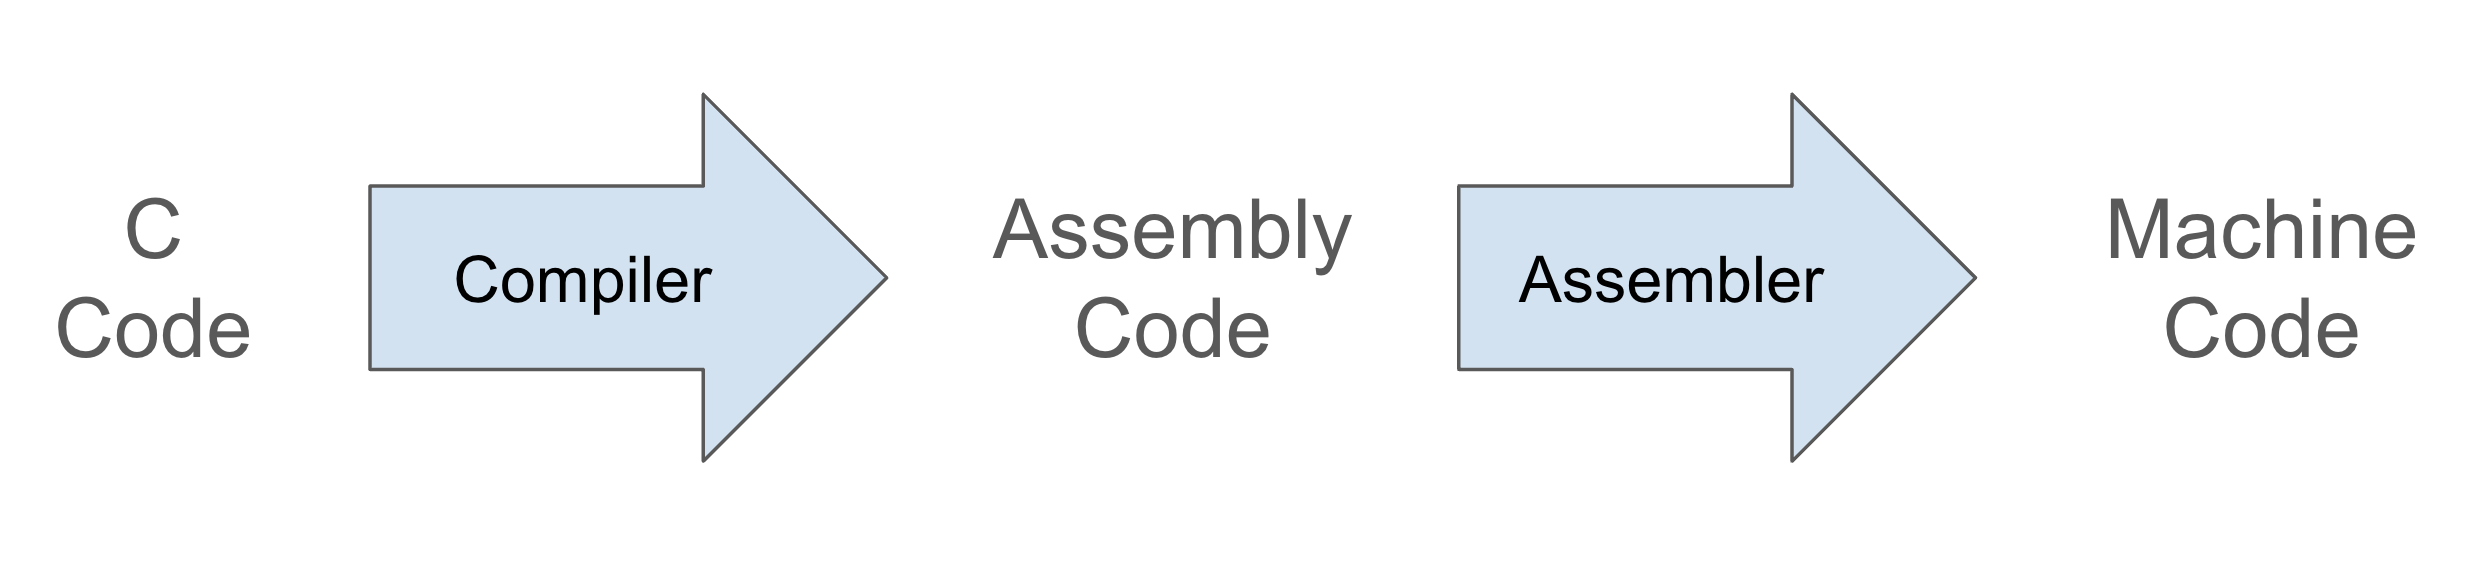
\includegraphics[width=\textwidth]{toolchain-flow.png}
\caption[\texorpdfstring{Toolchain Flow}{Toolchain Flow}]{\texorpdfstring{Toolchain flow from C source to \texttt{.memb} memory image and hardware simulation}{Toolchain flow from C source to .memb memory image and hardware simulation}}
\label{fig:toolchain-flow}
\end{figure}

The compiler accepts a deliberately restricted C subset and emits assembly for
the custom ISA. The assembler then resolves labels, encodes instructions, and
lays out the final memory image for simulation. This separation is useful both
conceptually and practically. Compiler bugs can be distinguished from encoding
bugs, and emitted assembly can be inspected directly during debugging.

\section{Supported Source Language}

The compiler targets a compact subset of C centered on integer computation and
structured control flow. The currently supported source constructs are:

\begin{itemize}
    \item Integer scalar declarations such as \texttt{int x;} and
          \texttt{int x = expr;}
    \item One-dimensional integer arrays such as \texttt{int a[4];}
    \item Assignments to scalars and array elements
    \item Integer literals, variables, array indexing, and function calls
    \item Unary negation, represented internally as subtraction from zero
    \item Binary operators \texttt{+}, \texttt{-}, \texttt{\&}, and \texttt{|}
    \item Conditions using \texttt{==}, \texttt{!=}, \texttt{<},
          \texttt{<=}, \texttt{>}, and \texttt{>=}
    \item \texttt{if}/\texttt{else}, \texttt{while}, and \texttt{for}
    \item Function parameters passed by value or by pointer
\end{itemize}

The compiler is intentionally not a full C implementation. Important omissions
include preprocessing, multiple translation units, data types other than
\texttt{int}, block-scoped shadowing, general pointer arithmetic, recursion,
and value-producing relational expressions such as \texttt{x = a < b;}.

\section{Compiler Pipeline}

The compiler implementation is organized as a simple multi-stage pipeline.

\subsection{Lexing and Parsing}

The front end first strips line comments and tokenizes identifiers, integer
literals, punctuation, arithmetic and bitwise operators, and relational
operators. A hand-written recursive-descent parser then constructs an abstract
syntax tree (AST) representing declarations, expressions, statements,
functions, and program structure.

Expression precedence is handled by layered parsing functions. This is
sufficient for the supported subset and keeps the implementation small enough
to study directly.

\begin{figure}[!htbp]
\centering
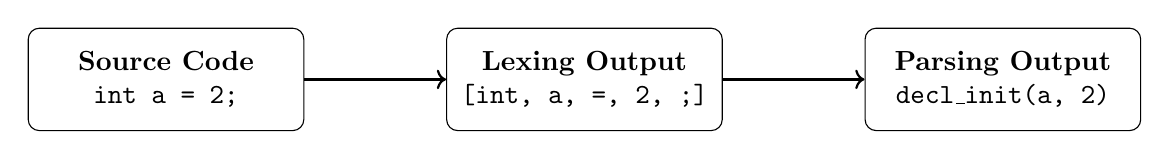
\begin{tikzpicture}[
    node distance=1.8cm,
    box/.style={
        draw,
        rectangle,
        rounded corners,
        minimum width=3.5cm,
        minimum height=1.3cm,
        align=center
    },
    arrow/.style={->, thick}
]

\node[box] (source) {
\textbf{Source Code} \\
\texttt{int a = 2;}
};

\node[box, right=of source] (lexer) {
\textbf{Lexing Output} \\
\texttt{[int, a, =, 2, ;]}
};

\node[box, right=of lexer] (parser) {
\textbf{Parsing Output} \\
\texttt{decl\_init(a, 2)}
};

\draw[arrow] (source) -- (lexer);
\draw[arrow] (lexer) -- (parser);

\end{tikzpicture}
\caption{Simplified lexing and parsing example}
\label{fig:lex-parse}
\end{figure}

The following excerpt, taken from
\href{https://github.com/shorewind/Custom-ISA-Toolchain/blob/main/compile.py}{compile.py}
(reproduced in Appendix~\ref{app:compile-py}), shows the actual lexer used in
the compiler:

\begin{center}
\begin{minipage}{0.88\textwidth}
\begin{lstlisting}[language=Python]
TOKEN_RE = re.compile(
    r"\s*(<=|>=|==|!=|[A-Za-z_]\w*|\d+|[{}()\[\];,+\-=&|<>*])"
)

def lex(src: str) -> List[str]:
    src = re.sub(r"//.*", "", src)
    toks: List[str] = []
    pos = 0
    while pos < len(src):
        m = TOKEN_RE.match(src, pos)
        if not m:
            if src[pos].isspace():
                pos += 1
                continue
            raise SyntaxError(f"Unexpected character at offset {pos}: {src[pos]!r}")
        toks.append(m.group(1))
        pos = m.end()
    return toks
\end{lstlisting}
\end{minipage}
\end{center}

This code reflects the deliberate scope of the language. The token set is
small, comments are removed before parsing, and invalid characters are rejected
early with a syntax error.

\subsection{TACKY-Style Intermediate Representation}

After parsing, the compiler lowers expressions into a simple linear
intermediate representation (IR) similar to the TACKY style described in
compiler-construction literature, particularly Nora Sandler's
\textit{Writing a C Compiler}~\cite{ref:sandler}. Here, TACKY refers to a tiny abstract
computer-like kernel representation in which complex expressions are broken
into simple, ordered steps. The purpose of this layer is not
optimization. Instead, it makes evaluation order explicit and prevents nested
expressions from accidentally clobbering intermediate values during code
generation.

For example, the supported expression
\begin{center}
\begin{minipage}{0.52\textwidth}
\begin{lstlisting}[language=C]
g = (a - b) & (a | b);
\end{lstlisting}
\end{minipage}
\end{center}

is lowered conceptually into:
\begin{center}
\begin{minipage}{0.35\textwidth}
\begin{lstlisting}[language=C]
t0 = a - b
t1 = a | b
g  = t0 & t1
\end{lstlisting}
\end{minipage}
\end{center}

\begin{figure}[!htbp]
\centering
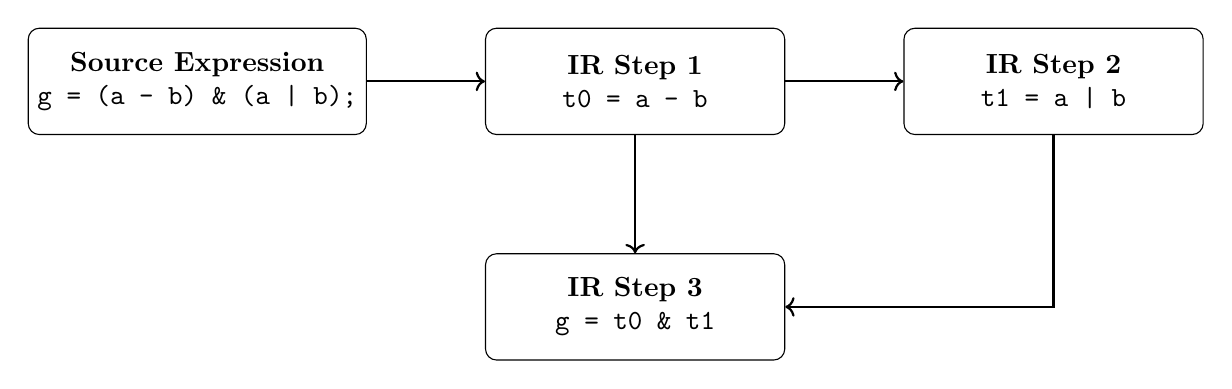
\begin{tikzpicture}[
    node distance=1.5cm,
    box/.style={
        draw,
        rectangle,
        rounded corners,
        minimum width=3.8cm,
        minimum height=1.35cm,
        align=center
    },
    arrow/.style={->, thick}
]

\node[box] (expr) {
\textbf{Source Expression} \\
\texttt{g = (a - b) \& (a | b);}
};

\node[box, right=of expr] (ir) {
\textbf{IR Step 1} \\
\texttt{t0 = a - b}
};

\node[box, right=of ir] (codegen) {
\textbf{IR Step 2} \\
\texttt{t1 = a | b}
};

\node[box, below=of ir] (finalir) {
\textbf{IR Step 3} \\
\texttt{g = t0 \& t1}
};

\draw[arrow] (expr) -- (ir);
\draw[arrow] (ir) -- (codegen);
\draw[arrow] (ir) -- (finalir);
\draw[arrow] (codegen) |- (finalir);

\end{tikzpicture}
\caption{Simplified IR lowering example}
\label{fig:ir-lowering}
\end{figure}

This representation is especially valuable on a small ISA with limited scratch
registers. By forcing subexpressions to become named temporaries, the backend
can translate each step into a short assembly sequence without losing
correctness.

\subsection{Storage Model}

A central design decision is that source-level storage lives in memory rather
than in registers. Global variables, local variables, parameters, pointer
slots, array elements, and IR temporaries are all assigned labels in the
\texttt{.data} section. Registers are used only as short-lived scratch space
while emitting individual instruction sequences.

This design keeps the compiler simple and avoids the need for stack-frame
management or register allocation. It also has direct consequences:

\begin{itemize}
    \item Recursion and reentrant calls are not supported.
    \item Function arguments are copied into statically allocated parameter
          slots.
    \item Generated code performs more loads and stores than an optimizing
          compiler would.
    \item The assembly is easy to inspect because most named values correspond
          to visible \texttt{.data} labels.
\end{itemize}

\subsection{Register Usage in Generated Code}

Although the ISA itself does not enforce a calling convention, the compiler
uses a consistent scratch-register convention during code generation, shown in
Table~\ref{tab:codegen-regs}.

\begin{table}[!htbp]
\centering
\begin{tabular}{cl}
\toprule
\textbf{Register} & \textbf{Compiler usage} \\
\midrule
\texttt{r0} & Constant zero; base register for symbolic addresses; unconditional branch helper \\
\texttt{r1} & Primary operand register and function return value \\
\texttt{r2} & Secondary operand register or computed index value \\
\texttt{r3} & Result register and general staging scratch register \\
\texttt{r4} & Computed array-element address register \\
\texttt{r5} & Pointer and address scratch register \\
\texttt{r6} & Reserved scratch space for future backend expansion \\
\texttt{r7} & Link register for \texttt{JL}/\texttt{JR} \\
\bottomrule
\end{tabular}
\caption{Register usage convention in generated assembly}
\label{tab:codegen-regs}
\end{table}

\subsection{Function Calls and Pointer Parameters}

Function calls are implemented using statically allocated parameter slots and
the link register \texttt{r7}. For a pass-by-value call, the caller evaluates
each argument, stores it into the callee's parameter label, executes
\texttt{JL r7, callee}, and then uses \texttt{r1} as the returned value. For a
pointer parameter, the caller passes the address of a variable by loading a
helper label such as \nolinkurl{addr_main_a} and storing that address into the
callee's pointer slot. Inside the callee, dereference operations explicitly
load through the pointer.

The backend also supports nested non-recursive calls by saving \texttt{r7} into
a statically allocated memory slot when a function itself needs to call another
function. This is a practical compromise that preserves correctness without
introducing a stack.

The actual call-emission logic from
\href{https://github.com/shorewind/Custom-ISA-Toolchain/blob/main/compile.py}{compile.py}
(Appendix~\ref{app:compile-py}) appears below:

\begin{center}
\begin{minipage}{0.82\textwidth}
\begin{lstlisting}[language=Python]
for p, a in zip(callee_fn.params, args):
    self.emit_load_operand(fn, a, "r3")
    slot = self.lookup_symbol(callee, p.name).label
    self.emit(f"    ST    r3, {slot}(r0)")

if self.fn_needs_saved_r7.get(fn, False):
    saved_lbl = self.fn_saved_r7_label(fn)
    self.emit(f"    ST    r7, {saved_lbl}(r0)")
self.emit(f"    JL    r7, {callee}")
if self.fn_needs_saved_r7.get(fn, False):
    self.emit(f"    LD    r7, {saved_lbl}(r0)")

if instr.dst is not None:
    self.emit_store_scalar(fn, instr.dst, "r1")
\end{lstlisting}
\end{minipage}
\end{center}

This excerpt makes the calling convention concrete: argument values are written
to statically allocated slots, \texttt{JL} transfers control, \texttt{r7} is
preserved when necessary, and the return value comes back in \texttt{r1}.

\section{Assembler Design}

The assembler implementation follows a conventional two-pass design.

\begin{figure}[!htbp]
\centering
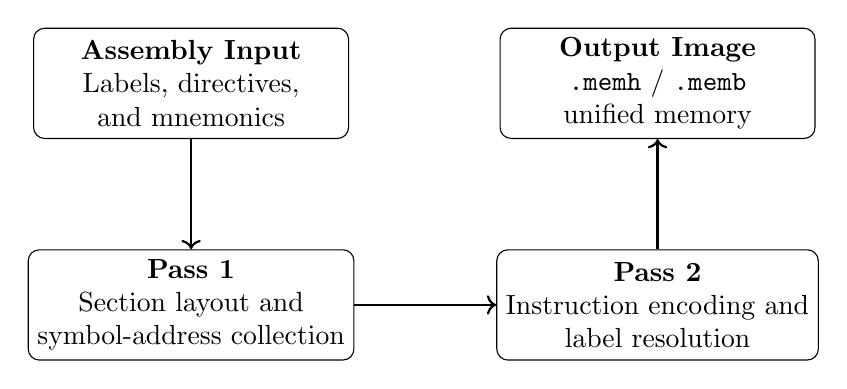
\begin{tikzpicture}[
    node distance=1.4cm and 1.8cm,
    box/.style={
        draw,
        rectangle,
        rounded corners,
        minimum width=4.0cm,
        minimum height=1.4cm,
        align=center
    },
    arrow/.style={->, thick}
]

\node[box] (asm) {
\textbf{Assembly Input} \\
Labels, directives, \\
and mnemonics
};

\node[box, below=of asm] (pass1) {
\textbf{Pass 1} \\
Section layout and \\
symbol-address collection
};

\node[box, right=of pass1] (pass2) {
\textbf{Pass 2} \\
Instruction encoding and \\
label resolution
};

\node[box, above=of pass2] (mem) {
\textbf{Output Image} \\
\texttt{.memh} / \texttt{.memb} \\
unified memory
};

\draw[arrow] (asm) -- (pass1);
\draw[arrow] (pass1) -- (pass2);
\draw[arrow] (pass2) -- (mem);

\end{tikzpicture}
\caption{Simplified two-pass assembler flow}
\label{fig:assembler-two-pass}
\end{figure}

\subsection{Pass 1: Symbol Resolution and Layout}

During the first pass, the assembler scans the source file, tracks whether it
is currently in \texttt{.text} or \texttt{.data}, records label addresses, and
counts instructions and data words. If a separate data base address is not
specified, the \texttt{.data} section begins immediately after the emitted text
section. In the current toolchain, \nolinkurl{text_base} defaults to 0, so the
base address of \texttt{.data} is determined as:
\begin{center}
\nolinkurl{data_base = text_base + count_text_words(lines)}
\end{center}
In other words, the first data word is placed at the word address equal to the
number of emitted instructions. This means that the final layout is compact and
depends directly on the number of instructions generated for each program.

The following excerpt from
\href{https://github.com/shorewind/Custom-ISA-Toolchain/blob/main/assemble.py}{assemble.py}
(Appendix~\ref{app:assemble-py}) shows the placement rule directly:

\begin{center}
\begin{minipage}{0.80\textwidth}
\begin{lstlisting}[language=Python]
def first_pass(
    lines: List[str],
    text_base: int = 0,
    data_base: Optional[int] = None,
) -> Tuple[List[Line], Dict[str, int]]:
    if data_base is None:
        data_base = text_base + count_text_words(lines)

    section = "text"
    pc_text = 0
    pc_data = 0
    sym: Dict[str, int] = {}
    parsed: List[Line] = []
\end{lstlisting}
\end{minipage}
\end{center}

This is the reason the report describes \texttt{.data} as starting immediately
after \texttt{.text}: that rule is not theoretical, but encoded explicitly in
the assembler. If a program contains 14 instructions, for example, the first
\texttt{.data} word is placed at address 14.

\subsection{Pass 2: Encoding}

In the second pass, mnemonics are mapped to opcodes and function codes,
register names are encoded, signed immediates are range-checked, branch offsets
are resolved relative to the current program counter, and jump targets are
encoded in absolute form. The result is a unified array of 1024 16-bit words.

The immediate-range check in
\href{https://github.com/shorewind/Custom-ISA-Toolchain/blob/main/assemble.py}{assemble.py}
(Appendix~\ref{app:assemble-py}) is implemented as follows:

\begin{center}
\begin{minipage}{0.70\textwidth}
\begin{lstlisting}[language=Python]
def to_twos_comp(val: int, bits: int) -> int:
    lo = -(1 << (bits - 1))
    hi = (1 << (bits - 1)) - 1
    if not (lo <= val <= hi):
        raise ValueError(
            f"Immediate {val} out of range for signed {bits}-bit ({lo} to {hi})."
        )
    return val & ((1 << bits) - 1)
\end{lstlisting}
\end{minipage}
\end{center}

This check is important because the ISA uses several signed immediate widths.
Rather than silently truncating values, the assembler rejects encodings that do
not fit the selected instruction format.

\subsection{Output Artifacts}

The assembler produces machine-code memory images in two textual forms:
\texttt{.memh} and \texttt{.memb}. The \texttt{.memh} form stores each 16-bit
word in hexadecimal and is typically paired with Verilog's
\texttt{\$readmemh}. The \texttt{.memb} form stores the same memory image in
binary and pairs naturally with \texttt{\$readmemb}. Both forms encode the
same program and data. This report uses \texttt{.memb} throughout the
compilation examples because it exposes the full instruction bit patterns more
directly, while \texttt{.memh} remains useful for compact inspection and for
testbenches that expect hexadecimal input. Because the memory image spans the
full architectural address space, unused locations are zero-filled.

\section{Memory Image}

Two details of the current implementation are important for interpreting the
generated memory image.

\begin{itemize}
    \item The memory image is 1024 words deep, matching the ISA model used by
          both the assembler and the automated behavior tests.
    \item The assembler records labels such as \texttt{main} but does not
          insert a startup stub. Hardware that begins execution at address zero
          must either have \texttt{main} located first in the text section or
          explicitly start from the address associated with \texttt{main}.
\end{itemize}

\section{Validation Workflow}

The implementation uses two complementary styles of validation.

\begin{itemize}
    \item Artifact-based fixtures grouped by expressions, arrays, control flow,
          and function calls allow emitted assembly and memory images to be
          inspected directly.
    \item A semantic unit-test harness compiles, assembles, and executes small
          programs inside a Python ISA interpreter so that behavioral
          correctness can be checked end-to-end.
\end{itemize}

Together, these methods make it possible to debug both code generation format
and actual program meaning.

\chapter{Examples and Feature Coverage}

This chapter presents the full feature-check suite used to demonstrate the supported language features of the completed toolchain. The examples are organized by expressions, arrays, control flow, and function calls. For each functionality example, the C source, the full generated assembly file, and the generated machine code are shown. The machine-code listings are presented in \texttt{.memb} format with explicit word addresses and stop at the last word belonging to the program's \texttt{.data} section, so trailing zero-filled memory beyond the program image is omitted. The corresponding fixture files are stored under \href{https://github.com/shorewind/Custom-ISA-Toolchain/tree/main/tests/feature-check}{tests/feature-check} in the repository.

\section{Arithmetic Operations}
Reference files:
\href{https://github.com/shorewind/Custom-ISA-Toolchain/blob/main/tests/feature-check/expressions/arithmetic.c}{C source},
\href{https://github.com/shorewind/Custom-ISA-Toolchain/blob/main/tests/feature-check/expressions/arithmetic.s}{assembly},
\href{https://github.com/shorewind/Custom-ISA-Toolchain/blob/main/tests/feature-check/expressions/arithmetic.memb}{machine code}.

\subsection*{C source}
\begin{lstlisting}[language=C]
int g;

int main() {
    int a = 5;
    int b = 2;

    g = (a - b) & (a | b);
    return g;
}
\end{lstlisting}

\subsection*{Generated assembly}
\begin{lstlisting}[language=CustomISAAsm]
.text
.global main

main:
    LD    r1, main_a(r0)
    LD    r2, main_b(r0)
    SUB   r3, r1, r2
    ST    r3, main_t0(r0)
    LD    r1, main_a(r0)
    LD    r2, main_b(r0)
    OR    r3, r1, r2
    ST    r3, main_t1(r0)
    LD    r1, main_t0(r0)
    LD    r2, main_t1(r0)
    AND   r3, r1, r2
    ST    r3, g(r0)
    LD    r1, g(r0)
    HALT

.data
g: .word 0
main_a: .word 5
main_b: .word 2
main_t0: .word 0
main_t1: .word 0
\end{lstlisting}

\subsection*{Generated machine code (.memb, addressed through .data)}
\begin{lstlisting}
0000: 0100000010001111
0001: 0100000100010000
0002: 0000010100110010
0003: 0010000110010001
0004: 0100000010001111
0005: 0100000100010000
0006: 0000010100110110
0007: 0010000110010010
0008: 0100000010010001
0009: 0100000100010010
0010: 0000010100110100
0011: 0010000110001110
0012: 0100000010001110
0013: 0000000000001110
0014: 0000000000000000
0015: 0000000000000101
0016: 0000000000000010
0017: 0000000000000000
0018: 0000000000000000
\end{lstlisting}

This example shows how arithmetic and bitwise expressions are translated into a sequence of simple operations. The compiler preserves evaluation order by storing intermediate results in temporary memory locations before combining them in the final operation.

\section{Static Array Access}
Reference files:
\href{https://github.com/shorewind/Custom-ISA-Toolchain/blob/main/tests/feature-check/arrays/array-static.c}{C source},
\href{https://github.com/shorewind/Custom-ISA-Toolchain/blob/main/tests/feature-check/arrays/array-static.s}{assembly},
\href{https://github.com/shorewind/Custom-ISA-Toolchain/blob/main/tests/feature-check/arrays/array-static.memb}{machine code}.

\subsection*{C source}
\begin{lstlisting}[language=C]
int g;
int a[2];

int main() {
    a[0] = 1;
    a[1] = 2;

    g = a[0] + a[1];
    return g;
}
\end{lstlisting}

\subsection*{Generated assembly}
\begin{lstlisting}[language=CustomISAAsm]
.text
.global main

main:
    LDI   r3, 1
    ST    r3, a(r0)
    LDI   r3, 2
    ST    r3, a+1(r0)
    LD    r3, a(r0)
    ST    r3, main_t0(r0)
    LD    r3, a+1(r0)
    ST    r3, main_t1(r0)
    LD    r1, main_t0(r0)
    LD    r2, main_t1(r0)
    ADD   r3, r1, r2
    ST    r3, g(r0)
    LD    r1, g(r0)
    HALT

.data
g: .word 0
a: .word 0
a_1: .word 0
main_t0: .word 0
main_t1: .word 0
\end{lstlisting}

\subsection*{Generated machine code (.memb, addressed through .data)}
\begin{lstlisting}
0000: 0110110000000001
0001: 0010000110001111
0002: 0110110000000010
0003: 0010000110010000
0004: 0100000110001111
0005: 0010000110010001
0006: 0100000110010000
0007: 0010000110010010
0008: 0100000010010001
0009: 0100000100010010
0010: 0000010100110000
0011: 0010000110001110
0012: 0100000010001110
0013: 0000000000001110
0014: 0000000000000000
0015: 0000000000000000
0016: 0000000000000000
0017: 0000000000000000
0018: 0000000000000000
\end{lstlisting}

This example shows the constant-index array case. Because the indices are known in advance, the generated assembly can access array elements directly through fixed symbolic offsets rather than computing element addresses at runtime.

\section{Dynamic Array Access}
Reference files:
\href{https://github.com/shorewind/Custom-ISA-Toolchain/blob/main/tests/feature-check/arrays/array-dynamic.c}{C source},
\href{https://github.com/shorewind/Custom-ISA-Toolchain/blob/main/tests/feature-check/arrays/array-dynamic.s}{assembly},
\href{https://github.com/shorewind/Custom-ISA-Toolchain/blob/main/tests/feature-check/arrays/array-dynamic.memb}{machine code}.

\subsection*{C source}
\begin{lstlisting}[language=C]
int a[4];

int main() {
    int i = 1;

    a[i + 1] = 9;
    return a[i + 1];
}
\end{lstlisting}

\subsection*{Generated assembly}
\begin{lstlisting}[language=CustomISAAsm]
.text
.global main

main:
    LD    r1, main_i(r0)
    LDI   r2, 1
    ADD   r3, r1, r2
    ST    r3, main_t0(r0)
    LD    r5, addr_a(r0)
    LD    r2, main_t0(r0)
    ADD   r4, r5, r2
    LDI   r3, 9
    ST    r3, 0(r4)
    LD    r1, main_i(r0)
    LDI   r2, 1
    ADD   r3, r1, r2
    ST    r3, main_t1(r0)
    LD    r5, addr_a(r0)
    LD    r2, main_t1(r0)
    ADD   r4, r5, r2
    LD    r3, 0(r4)
    ST    r3, main_t2(r0)
    LD    r1, main_t2(r0)
    HALT

.data
a: .word 0
a_1: .word 0
a_2: .word 0
a_3: .word 0
main_i: .word 1
main_t0: .word 0
main_t1: .word 0
main_t2: .word 0
addr_a: .word a
\end{lstlisting}

\subsection*{Generated machine code (.memb, addressed through .data)}
\begin{lstlisting}
0000: 0100000010011000
0001: 0110100000000001
0002: 0000010100110000
0003: 0010000110011001
0004: 0100001010011100
0005: 0100000100011001
0006: 0001010101000000
0007: 0110110000001001
0008: 0011000110000000
0009: 0100000010011000
0010: 0110100000000001
0011: 0000010100110000
0012: 0010000110011010
0013: 0100001010011100
0014: 0100000100011010
0015: 0001010101000000
0016: 0101000110000000
0017: 0010000110011011
0018: 0100000010011011
0019: 0000000000001110
0020: 0000000000000000
0021: 0000000000000000
0022: 0000000000000000
0023: 0000000000000000
0024: 0000000000000001
0025: 0000000000000000
0026: 0000000000000000
0027: 0000000000000000
0028: 0000000000010100
\end{lstlisting}

This example shows how computed indices are handled. Because the target instruction set architecture has no scaled indexed addressing mode, the compiler computes the index expression explicitly, loads the array base address from a helper label, and forms the final element address before the load or store.

\section{Conditional If/Else Statement}
Reference files:
\href{https://github.com/shorewind/Custom-ISA-Toolchain/blob/main/tests/feature-check/control-flow/if-else-geq.c}{C source},
\href{https://github.com/shorewind/Custom-ISA-Toolchain/blob/main/tests/feature-check/control-flow/if-else-geq.s}{assembly},
\href{https://github.com/shorewind/Custom-ISA-Toolchain/blob/main/tests/feature-check/control-flow/if-else-geq.memb}{machine code}.

\subsection*{C source}
\begin{lstlisting}[language=C]
int g;

int main() {
    int a = 1;

    if (a >= 1) {
        g = 7;
    } else {
        g = 3;
    }

    return g;
}
\end{lstlisting}

\subsection*{Generated assembly}
\begin{lstlisting}[language=CustomISAAsm]
.text
.global main

main:
    LD    r1, main_a(r0)
    LDI   r2, 1
    SLT   r3, r1, r2
    BNZ   r3, if_else_1
    LDI   r3, 7
    ST    r3, g(r0)
    BEZ   r0, if_end_1
if_else_1:
    LDI   r3, 3
    ST    r3, g(r0)
if_end_1:
    LD    r1, g(r0)
    HALT

.data
g: .word 0
main_a: .word 1
\end{lstlisting}

\subsection*{Generated machine code (.memb, addressed through .data)}
\begin{lstlisting}
0000: 0100000010001100
0001: 0110100000000001
0002: 0000010100111000
0003: 1010110000000011
0004: 0110110000000111
0005: 0010000110001011
0006: 1000000000000010
0007: 0110110000000011
0008: 0010000110001011
0009: 0100000010001011
0010: 0000000000001110
0011: 0000000000000000
0012: 0000000000000001
\end{lstlisting}

This example shows conditional branching using the greater-than-or-equal relation. The comparison is lowered into a set-less-than instruction and a conditional branch, which selects between the then path and the else path.

\section{While Loop}
Reference files:
\href{https://github.com/shorewind/Custom-ISA-Toolchain/blob/main/tests/feature-check/control-flow/while-lt.c}{C source},
\href{https://github.com/shorewind/Custom-ISA-Toolchain/blob/main/tests/feature-check/control-flow/while-lt.s}{assembly},
\href{https://github.com/shorewind/Custom-ISA-Toolchain/blob/main/tests/feature-check/control-flow/while-lt.memb}{machine code}.

\subsection*{C source}
\begin{lstlisting}[language=C]
int g;

int main() {
    int i = 0;
    int s = 0;

    while (i < 2) {
        s = s + i;
        i = i + 1;
    }

    g = s;
    return g;
}
\end{lstlisting}

\subsection*{Generated assembly}
\begin{lstlisting}[language=CustomISAAsm]
.text
.global main

main:
while_start_1:
    LD    r1, main_i(r0)
    LDI   r2, 2
    SLT   r3, r1, r2
    BEZ   r3, while_end_1
    LD    r1, main_s(r0)
    LD    r2, main_i(r0)
    ADD   r3, r1, r2
    ST    r3, main_s(r0)
    LD    r1, main_i(r0)
    LDI   r2, 1
    ADD   r3, r1, r2
    ST    r3, main_i(r0)
    BEZ   r0, while_start_1
while_end_1:
    LD    r3, main_s(r0)
    ST    r3, g(r0)
    LD    r1, g(r0)
    HALT

.data
g: .word 0
main_i: .word 0
main_s: .word 0
\end{lstlisting}

\subsection*{Generated machine code (.memb, addressed through .data)}
\begin{lstlisting}
0000: 0100000010010010
0001: 0110100000000010
0002: 0000010100111000
0003: 1000110000001001
0004: 0100000010010011
0005: 0100000100010010
0006: 0000010100110000
0007: 0010000110010011
0008: 0100000010010010
0009: 0110100000000001
0010: 0000010100110000
0011: 0010000110010010
0012: 1000001111110011
0013: 0100000110010011
0014: 0010000110010001
0015: 0100000010010001
0016: 0000000000001110
0017: 0000000000000000
0018: 0000000000000000
0019: 0000000000000000
\end{lstlisting}

This example shows a loop header, a loop-exit test, and a loop back-edge. The generated code reevaluates the loop condition on each iteration and branches back to the loop start until the condition becomes false.

\section{For Loop}
Reference files:
\href{https://github.com/shorewind/Custom-ISA-Toolchain/blob/main/tests/feature-check/control-flow/for-leq.c}{C source},
\href{https://github.com/shorewind/Custom-ISA-Toolchain/blob/main/tests/feature-check/control-flow/for-leq.s}{assembly},
\href{https://github.com/shorewind/Custom-ISA-Toolchain/blob/main/tests/feature-check/control-flow/for-leq.memb}{machine code}.

\subsection*{C source}
\begin{lstlisting}[language=C]
int g;

int main() {
    int i = 0;
    int s = 0;

    for (i = 0; i <= 1; i = i + 1) {
        s = i;
    }

    g = s;
    return g;
}
\end{lstlisting}

\subsection*{Generated assembly}
\begin{lstlisting}[language=CustomISAAsm]
.text
.global main

main:
    LDI   r3, 0
    ST    r3, main_i(r0)
for_start_1:
    LD    r1, main_i(r0)
    LDI   r2, 1
    SLT   r3, r2, r1
    BNZ   r3, for_end_1
    LD    r3, main_i(r0)
    ST    r3, main_s(r0)
    LD    r1, main_i(r0)
    LDI   r2, 1
    ADD   r3, r1, r2
    ST    r3, main_i(r0)
    BEZ   r0, for_start_1
for_end_1:
    LD    r3, main_s(r0)
    ST    r3, g(r0)
    LD    r1, g(r0)
    HALT

.data
g: .word 0
main_i: .word 0
main_s: .word 0
\end{lstlisting}

\subsection*{Generated machine code (.memb, addressed through .data)}
\begin{lstlisting}
0000: 0110110000000000
0001: 0010000110010010
0002: 0100000010010010
0003: 0110100000000001
0004: 0000100010111000
0005: 1010110000000111
0006: 0100000110010010
0007: 0010000110010011
0008: 0100000010010010
0009: 0110100000000001
0010: 0000010100110000
0011: 0010000110010010
0012: 1000001111110101
0013: 0100000110010011
0014: 0010000110010001
0015: 0100000010010001
0016: 0000000000001110
0017: 0000000000000000
0018: 0000000000000000
0019: 0000000000000000
\end{lstlisting}

This example shows a for loop with explicit initialization, comparison, update, and exit behavior. It is useful because it demonstrates how the less-than-or-equal relation is implemented using the available comparison and branch instructions.

\section{For Loop with Declaration}
Reference files:
\href{https://github.com/shorewind/Custom-ISA-Toolchain/blob/main/tests/feature-check/control-flow/for-init-decl.c}{C source},
\href{https://github.com/shorewind/Custom-ISA-Toolchain/blob/main/tests/feature-check/control-flow/for-init-decl.s}{assembly},
\href{https://github.com/shorewind/Custom-ISA-Toolchain/blob/main/tests/feature-check/control-flow/for-init-decl.memb}{machine code}.

\subsection*{C source}
\begin{lstlisting}[language=C]
int main() {
    int s = 0;

    for (int i = 0; i < 3; i = i + 1) {
        s = s + 1;
    }

    return s;
}
\end{lstlisting}

\subsection*{Generated assembly}
\begin{lstlisting}[language=CustomISAAsm]
.text
.global main

main:
for_start_1:
    LD    r1, main_i(r0)
    LDI   r2, 3
    SLT   r3, r1, r2
    BEZ   r3, for_end_1
    LD    r1, main_s(r0)
    LDI   r2, 1
    ADD   r3, r1, r2
    ST    r3, main_s(r0)
    LD    r1, main_i(r0)
    LDI   r2, 1
    ADD   r3, r1, r2
    ST    r3, main_i(r0)
    BEZ   r0, for_start_1
for_end_1:
    LD    r1, main_s(r0)
    HALT

.data
main_s: .word 0
main_i: .word 0
\end{lstlisting}

\subsection*{Generated machine code (.memb, addressed through .data)}
\begin{lstlisting}
0000: 0100000010010000
0001: 0110100000000011
0002: 0000010100111000
0003: 1000110000001001
0004: 0100000010001111
0005: 0110100000000001
0006: 0000010100110000
0007: 0010000110001111
0008: 0100000010010000
0009: 0110100000000001
0010: 0000010100110000
0011: 0010000110010000
0012: 1000001111110011
0013: 0100000010001111
0014: 0000000000001110
0015: 0000000000000000
0016: 0000000000000000
\end{lstlisting}

This example shows that a declaration in the initialization clause of a for loop is handled correctly. The generated code includes the loop control variable as a normal stored value in the data region and updates it explicitly on each iteration.

\section{Relational Operator Tests}
Reference files:
\href{https://github.com/shorewind/Custom-ISA-Toolchain/blob/main/tests/feature-check/control-flow/relops.c}{C source},
\href{https://github.com/shorewind/Custom-ISA-Toolchain/blob/main/tests/feature-check/control-flow/relops.s}{assembly},
\href{https://github.com/shorewind/Custom-ISA-Toolchain/blob/main/tests/feature-check/control-flow/relops.memb}{machine code}.

\subsection*{C source}
\begin{lstlisting}[language=C]
int g;

int main() {
    int a = 3;
    int b = 5;
    int r = 0;

    if (a == 3) {
        r = r + 1;
    }
    if (a != b) {
        r = r + 1;
    }
    if (b > a) {
        r = r + 1;
    }

    g = r;
    return g;
}
\end{lstlisting}

\subsection*{Generated assembly}
\begin{lstlisting}[language=CustomISAAsm]
.text
.global main

main:
    LD    r1, main_a(r0)
    LDI   r2, 3
    SUB   r3, r1, r2
    BNZ   r3, if_else_1
    LD    r1, main_r(r0)
    LDI   r2, 1
    ADD   r3, r1, r2
    ST    r3, main_r(r0)
    BEZ   r0, if_end_1
if_else_1:
if_end_1:
    LD    r1, main_a(r0)
    LD    r2, main_b(r0)
    SUB   r3, r1, r2
    BEZ   r3, if_else_2
    LD    r1, main_r(r0)
    LDI   r2, 1
    ADD   r3, r1, r2
    ST    r3, main_r(r0)
    BEZ   r0, if_end_2
if_else_2:
if_end_2:
    LD    r1, main_b(r0)
    LD    r2, main_a(r0)
    SLT   r3, r2, r1
    BEZ   r3, if_else_3
    LD    r1, main_r(r0)
    LDI   r2, 1
    ADD   r3, r1, r2
    ST    r3, main_r(r0)
    BEZ   r0, if_end_3
if_else_3:
if_end_3:
    LD    r3, main_r(r0)
    ST    r3, g(r0)
    LD    r1, g(r0)
    HALT

.data
g: .word 0
main_a: .word 3
main_b: .word 5
main_r: .word 0
\end{lstlisting}

\subsection*{Generated machine code (.memb, addressed through .data)}
\begin{lstlisting}
0000: 0100000010100000
0001: 0110100000000011
0002: 0000010100110010
0003: 1010110000000101
0004: 0100000010100010
0005: 0110100000000001
0006: 0000010100110000
0007: 0010000110100010
0008: 1000000000000000
0009: 0100000010100000
0010: 0100000100100001
0011: 0000010100110010
0012: 1000110000000101
0013: 0100000010100010
0014: 0110100000000001
0015: 0000010100110000
0016: 0010000110100010
0017: 1000000000000000
0018: 0100000010100001
0019: 0100000100100000
0020: 0000100010111000
0021: 1000110000000101
0022: 0100000010100010
0023: 0110100000000001
0024: 0000010100110000
0025: 0010000110100010
0026: 1000000000000000
0027: 0100000110100010
0028: 0010000110011111
0029: 0100000010011111
0030: 0000000000001110
0031: 0000000000000000
0032: 0000000000000011
0033: 0000000000000101
0034: 0000000000000000
\end{lstlisting}

This example collects several relational forms in one program. It shows how equality, inequality, and greater-than tests are each implemented using combinations of subtraction, set-less-than, and conditional branching.

\section{Pass-by-Value Function Call}
Reference files:
\href{https://github.com/shorewind/Custom-ISA-Toolchain/blob/main/tests/feature-check/calls/value-param.c}{C source},
\href{https://github.com/shorewind/Custom-ISA-Toolchain/blob/main/tests/feature-check/calls/value-param.s}{assembly},
\href{https://github.com/shorewind/Custom-ISA-Toolchain/blob/main/tests/feature-check/calls/value-param.memb}{machine code}.

\subsection*{C source}
\begin{lstlisting}[language=C]
int g;

int inc(int x) {
    x = x + 1;
    return x;
}

int main() {
    int a = 4;

    g = inc(a);
    return a;
}
\end{lstlisting}

\subsection*{Generated assembly}
\begin{lstlisting}[language=CustomISAAsm]
.text
.global main

inc:
    LD    r1, inc_p_val_x(r0)
    LDI   r2, 1
    ADD   r3, r1, r2
    ST    r3, inc_p_val_x(r0)
    LD    r1, inc_p_val_x(r0)
    JR    r7

main:
    LD    r3, main_a(r0)
    ST    r3, inc_p_val_x(r0)
    JL    r7, inc
    ST    r1, main_t0(r0)
    LD    r3, main_t0(r0)
    ST    r3, g(r0)
    LD    r1, main_a(r0)
    HALT

.data
g: .word 0
inc_p_val_x: .word 0
main_a: .word 4
main_t0: .word 0
\end{lstlisting}

\subsection*{Generated machine code (.memb, addressed through .data)}
\begin{lstlisting}
0000: 0100000010001111
0001: 0110100000000001
0002: 0000010100110000
0003: 0010000110001111
0004: 0100000010001111
0005: 1111110000000000
0006: 0100000110010000
0007: 0010000110001111
0008: 1101110000000000
0009: 0010000010010001
0010: 0100000110010001
0011: 0010000110001110
0012: 0100000010010000
0013: 0000000000001110
0014: 0000000000000000
0015: 0000000000000000
0016: 0000000000000100
0017: 0000000000000000
\end{lstlisting}

This example shows ordinary pass-by-value behavior. The caller copies the argument into the callee parameter slot, the callee operates on that copied value, and the caller's original variable remains unchanged after the call returns.

\section{Pass-by-Reference (Pointer) Function Call}
Reference files:
\href{https://github.com/shorewind/Custom-ISA-Toolchain/blob/main/tests/feature-check/calls/ptr-param.c}{C source},
\href{https://github.com/shorewind/Custom-ISA-Toolchain/blob/main/tests/feature-check/calls/ptr-param.s}{assembly},
\href{https://github.com/shorewind/Custom-ISA-Toolchain/blob/main/tests/feature-check/calls/ptr-param.memb}{machine code}.

\subsection*{C source}
\begin{lstlisting}[language=C]
int bump(int *x) {
    *x = *x + 1;
    return *x;
}

int main() {
    int a = 4;
    bump(&a);
    return a;
}
\end{lstlisting}

\subsection*{Generated assembly}
\begin{lstlisting}[language=CustomISAAsm]
.text
.global main

bump:
    LD    r5, bump_p_ptr_x(r0)
    LD    r3, 0(r5)
    ST    r3, bump_t0(r0)
    LD    r1, bump_t0(r0)
    LDI   r2, 1
    ADD   r3, r1, r2
    ST    r3, bump_t1(r0)
    LD    r3, bump_t1(r0)
    LD    r5, bump_p_ptr_x(r0)
    ST    r3, 0(r5)
    LD    r5, bump_p_ptr_x(r0)
    LD    r3, 0(r5)
    ST    r3, bump_t2(r0)
    LD    r1, bump_t2(r0)
    JR    r7

main:
    LD    r3, addr_main_a(r0)
    ST    r3, main_t0(r0)
    LD    r3, main_t0(r0)
    ST    r3, bump_p_ptr_x(r0)
    JL    r7, bump
    ST    r1, main_t1(r0)
    LD    r1, main_a(r0)
    HALT

.data
bump_p_ptr_x: .word 0
bump_t0: .word 0
bump_t1: .word 0
bump_t2: .word 0
main_a: .word 4
main_t0: .word 0
main_t1: .word 0
addr_main_a: .word main_a
\end{lstlisting}

\subsection*{Generated machine code (.memb, addressed through .data)}
\begin{lstlisting}
0000: 0100001010010111
0001: 0101010110000000
0002: 0010000110011000
0003: 0100000010011000
0004: 0110100000000001
0005: 0000010100110000
0006: 0010000110011001
0007: 0100000110011001
0008: 0100001010010111
0009: 0011010110000000
0010: 0100001010010111
0011: 0101010110000000
0012: 0010000110011010
0013: 0100000010011010
0014: 1111110000000000
0015: 0100000110011110
0016: 0010000110011100
0017: 0100000110011100
0018: 0010000110010111
0019: 1101110000000000
0020: 0010000010011101
0021: 0100000010011011
0022: 0000000000001110
0023: 0000000000000000
0024: 0000000000000000
0025: 0000000000000000
0026: 0000000000000000
0027: 0000000000000100
0028: 0000000000000000
0029: 0000000000000000
0030: 0000000000011011
\end{lstlisting}

This example shows pass-by-reference-style behavior implemented with pointers. The caller passes the address of a variable, and the callee explicitly dereferences that pointer to update caller-owned storage in memory.

Together, these examples provide full coverage of the feature-check suite used in this project. They demonstrate arithmetic and bitwise computation, constant-index and computed-index array access, structured control flow, multiple relational operators, pass-by-value calls, and pass-by-reference-style pointer calls. When combined with the automated behavior tests described in the next chapter, they provide strong evidence that the implemented toolchain supports the full C subset claimed in this report.

\chapter{Verification and Results}

The toolchain was validated in three complementary ways: by inspecting the
generated files, by running automated behavior tests, and by loading the
generated memory image into the hardware model.

\section{Checking the Generated Files}

The first level of validation was direct inspection of the generated outputs.
For each example program, the source file, generated assembly file, and
generated machine-code files were kept together. This makes it possible to
check whether the compiler and assembler are producing sensible results before
running the program.

In practice, this means a reader can verify behavior by checking whether:

\begin{itemize}
    \item a C statement is translated into the expected assembly sequence,
    \item labels and data objects appear in the expected places,
    \item the binary \texttt{.memb} file and hexadecimal \texttt{.memh} file
          match the generated assembly, and
    \item addresses in the final image line up with the instruction and
          \texttt{.data} layout described earlier in the report.
\end{itemize}

This form of checking is especially useful when debugging code generation
format, memory layout, and instruction encoding.

\section{Running Automated Behavior Tests}

The second level of validation was an automated Python test harness that checks
program meaning, not just file contents. Each test follows the same pipeline:

\begin{enumerate}
    \item Compile source text into assembly.
    \item Assemble the emitted program into a 1024-word image.
    \item Execute that image in a small Python interpreter for the custom ISA.
    \item Check the final return value and, where appropriate, the final memory state.
\end{enumerate}

This approach validates far more than parsing alone. It checks the lexer, the
parser, abstract syntax tree (AST) construction, intermediate representation
(IR) lowering, assembly generation, label resolution, machine-code encoding,
and the runtime behavior of the resulting program. The automated tests were
used to confirm:

\begin{itemize}
    \item Basic arithmetic correctness
    \item Preservation of left-hand subexpressions in nested expressions
    \item Correct dynamic array address generation
    \item Correct handling of nested function calls
    \item Correct mutation of caller-owned data through pointer parameters
\end{itemize}

The core of that harness in
\href{https://github.com/shorewind/Custom-ISA-Toolchain/blob/main/tests/test_compiler.py}{tests/test\_compiler.py}
(Appendix~\ref{app:test-compiler-py}) is concise:

\begin{center}
\begin{minipage}{0.74\textwidth}
\begin{lstlisting}[language=Python]
def compile_to_asm(src):
    tokens = ccompiler.lex(src)
    prog = ccompiler.Parser(tokens).parse_program()
    return ccompiler.CodeGen(prog).generate()

def assemble_text(asm):
    parsed, symbols = assemble.first_pass(asm.splitlines(), text_base=0)
    return assemble.second_pass(parsed, symbols, mem_depth=1024), symbols
\end{lstlisting}
\end{minipage}
\end{center}

This excerpt shows why the tests are meaningful: they use the real compiler and
the real assembler, not a separate mock implementation.

A user who wants to repeat this validation can run the test suite associated
with
\href{https://github.com/shorewind/Custom-ISA-Toolchain/blob/main/tests/test_compiler.py}{tests/test\_compiler.py}
(Appendix~\ref{app:test-compiler-py}) using:

\begin{center}
\begin{minipage}{0.60\textwidth}
\begin{lstlisting}
python3 -m unittest tests/test_compiler.py
\end{lstlisting}
\end{minipage}
\end{center}

They can also compile one example manually with
\href{https://github.com/shorewind/Custom-ISA-Toolchain/blob/main/build.py}{build.py}
(Appendix~\ref{app:build-py}) and inspect the outputs using:

\begin{center}
\begin{minipage}{0.32\textwidth}
\begin{lstlisting}
python3 build.py <input.c>
\end{lstlisting}
\end{minipage}
\end{center}

\section{Running the Hardware Model}

After assembly, the generated \texttt{.memb} image, or equivalently the same
image in \texttt{.memh} form, can be loaded directly into the processor's
unified memory for Verilog simulation. At this stage, the software toolchain
is no longer being checked in isolation. Instead, the full software-hardware
path is exercised:

\begin{itemize}
    \item instruction fetch from the emitted memory image
    \item control-unit decode of each encoded instruction
    \item ALU execution of arithmetic and relational operations
    \item memory reads and writes through the LS-format instructions
    \item control-flow changes caused by branches and jumps
    \item function call and return behavior through \texttt{JL} and \texttt{JR}
\end{itemize}

In the Questa FPGA simulation software, this validation can be carried out by creating and using a
testbench for the processor. The testbench is responsible for instantiating
the hardware design, providing clock and reset behavior, loading the generated
\texttt{.memb} or \texttt{.memh} memory image into the processor memory by
using a Verilog memory-loading system task such as \texttt{\$readmemb} or
\texttt{\$readmemh}, and allowing the design to execute for enough cycles to
complete the program. During simulation, waveform and variable views can be
used to observe the program counter, register file, arithmetic logic unit
behavior, control signals, and selected memory locations. Verification is then
performed by checking that the register values and memory states match the
expected behavior of the compiled program. The specific testbench used for this
validation, \texttt{tb\_cpu.v}, is reproduced in Appendix~\ref{app:tb-cpu}.

Because the processor is single-cycle, interpreting simulation results is
straightforward. Each clock cycle corresponds to one completed instruction, so
program-counter movement, register updates, and memory writes can be traced
directly back to the generated assembly.

In practical terms, a user can further verify the design by loading one of the
generated memory images into the processor testbench and checking that:

\begin{itemize}
    \item the program counter follows the expected instruction sequence,
    \item registers receive the expected intermediate and final values,
    \item memory locations in the \texttt{.data} region are updated correctly,
          and
    \item the processor halts with the expected return value in the designated
          return register.
\end{itemize}

\subsection{Arithmetic Example in Questa}
\label{sec:questa-arith}

To validate the simplest end-to-end hardware path, the arithmetic example from
the feature-check suite was loaded into the processor testbench implemented in
Appendix~\ref{app:tb-cpu}. For this run, the generated memory image was loaded
into the testbench memory as \texttt{test-case.memb}. The successful Questa
startup and design load were captured in \texttt{isa/simulate.txt}
(Appendix~\ref{app:sim-artifacts}), including:

\begin{center}
\begin{minipage}{0.88\textwidth}
\begin{lstlisting}
# Compile of cpu_toolchain_tb.v was successful.
Questa> vsim -t ns -voptargs=+acc work.tb_cpu
# Loading work.tb_cpu(fast)
# Loading work.cpu(fast)
\end{lstlisting}
\end{minipage}
\end{center}

The detailed execution trace and final register dump were captured in
\texttt{isa/output.txt} (Appendix~\ref{app:sim-artifacts}). The key point in
the trace is the final load of the computed result from memory location
\texttt{g} into return register \texttt{r1}:

\begin{center}
\begin{minipage}{0.88\textwidth}
\begin{lstlisting}
# ----- t=140 -----
# PC     = 12
# INSTR  = 0x408e
# WB     : write_reg=1 wb_data=3 reg_write=1
# REGS   : r0=0 r1=3 r2=7 r3=3 r4=0 r5=0 r6=0 r7=0
# MEM    : M[14]=3
# ----- t=150 -----
# PC     = 13
# INSTR  = 0x000e
# CONTROL: ... halt=1
\end{lstlisting}
\end{minipage}
\end{center}

This trace confirms the expected arithmetic result. By the time the processor
reaches \texttt{HALT}, register \texttt{r1} contains \texttt{3}, temporary
register \texttt{r3} also contains \texttt{3}, and memory address
\texttt{14}---the address of global \texttt{g} in this image---contains
\texttt{3}. The final register summary in \texttt{isa/output.txt} therefore
matches the expected post-execution state described earlier in the examples
chapter.

\section{Observed Outcomes}

Across the feature fixtures and automated behavior tests, the current toolchain
successfully demonstrates the targeted capabilities of the project:

\begin{itemize}
    \item arithmetic and bitwise computation on integer values
    \item scalar and array storage in a unified memory space
    \item structured control flow translated into labels and branches
    \item function calls using a link register and statically allocated parameter slots
    \item pointer-based mutation through explicit address passing and dereference
\end{itemize}

These results are sufficient to show that the toolchain is not merely producing
syntactically plausible assembly, but is preserving program meaning for the
supported source subset.

\chapter{Analysis}

\section{Limitations}

The system is intentionally small, and that simplicity comes with clear
limitations.

\begin{itemize}
    \item There is no runtime stack, so recursion and reentrant calls are not supported.
    \item Most source-level values live in memory, so the generated code performs many loads and stores.
    \item The language subset is narrow: only \texttt{int} values are supported, preprocessing is absent, and several ordinary C features are intentionally omitted.
    \item Relational operators are supported only inside conditions, not as general value-producing expressions.
    \item Program entry relies on the surrounding execution environment starting at \texttt{main} or placing \texttt{main} first in the text section.
\end{itemize}

Some of these limitations are architectural, while others are software design
choices made to keep the project understandable and tractable within the scope
of an undergraduate project.

\section{ISA Design Lessons}

One of the most important outcomes of the project is that building the
toolchain exposes practical strengths and weaknesses of the instruction set
architecture more clearly than hardware-only testing does.

\begin{itemize}
    \item \textbf{Immediate-width limits increase code size.} The existence of
          separate 3-bit, 7-bit, and 10-bit immediate fields is sufficient for
          a compact educational ISA, but it frequently forces the compiler to
          emit multiple instructions where a richer ISA could use one. This is
          especially visible in address setup, loop bounds, and constant
          materialization.
    \item \textbf{The lack of a stack strongly shapes the compiler design.}
          Because the exposed machine model does not provide a stack pointer or
          stack-frame discipline, the compiler stores locals, parameters, and
          temporaries in statically allocated memory. This keeps the backend
          simple, but it also prevents recursion and reentrant calls.
    \item \textbf{A small register file pushes the backend toward memory-heavy
          code generation.} With only a few practical scratch registers
          available, the compiler benefits from explicit temporaries in memory.
          The result is correct and easy to inspect, but not especially
          efficient.
    \item \textbf{Simple control flow is supported cleanly, but with limited
          flexibility.} The branch and jump instructions are sufficient for
          structured \texttt{if}, \texttt{while}, and \texttt{for} lowering.
          However, the simplicity of the control-flow model means that the
          assembler and compiler must do more work to manage labels, branch
          offsets, and call/return conventions explicitly.
    \item \textbf{The ISA is well suited to transparency and teaching.} Even
          when it is not optimized for compact code generation, the
          architecture's regular encoding and small instruction set make the
          translation from C source to assembly and machine code easy to follow.
\end{itemize}

Taken together, these lessons show that the architecture is successful as an
educational platform, but that extending it toward a more conventional software
environment would likely require improvements in addressing flexibility,
register resources, and runtime support.

\section{Future Work}

Several extensions would make the toolchain substantially more capable.

\begin{itemize}
    \item Add a stack pointer and call-frame discipline to support recursion and conventional local storage.
    \item Introduce register allocation so frequently used values can remain in registers longer.
    \item Expand the source-language subset with richer expressions, additional types, and better diagnostics.
    \item Add optimization passes such as constant folding, copy propagation, and dead-store elimination.
    \item Separate assembly, linking, and startup concerns so that program entry is explicit rather than assumed.
    \item Extend the hardware platform with more instructions or more flexible addressing modes to reduce backend complexity.
\end{itemize}

Each of these improvements would increase either expressiveness, performance, or
engineering robustness, but would also introduce additional implementation
complexity.

\chapter{Conclusion}

This project delivers a working compiler-assembler toolchain for a restricted
subset of C on a custom 16-bit processor. The result is a compact software
system that can translate nontrivial source programs into executable machine
code for the target architecture.

The most important outcome is not raw performance. Instead, the project shows
that a carefully chosen set of compiler techniques can be adapted to a very
small architectural target while still preserving clear program semantics. By
making evaluation order explicit, storing long-lived values in named memory
locations, and using a straightforward two-pass assembler, the design remains
small enough to understand while still supporting nontrivial programs with
arrays, control flow, and functions.

The project provides a practical demonstration of the relationship between
compiler construction, instruction-set design, and hardware execution. It
turns the ISA from an isolated hardware specification into a usable computing
environment.

\begin{thebibliography}{1}
\addcontentsline{toc}{chapter}{References}

\bibitem{ref:sandler}
N.~Sandler, \emph{Writing a C Compiler}. San Francisco, CA, USA: No Starch
Press, 2024.

\end{thebibliography}

\appendix
\chapter{Source Listings and Supporting Artifacts}

This appendix provides full copied source listings for the main software artifacts discussed in this report, along with selected simulation-support artifacts. For each file, a GitHub link is also provided so that the reader can compare the copied listing in this report against the current repository version.

\section{Repository Link}

The full project repository is available at:

\begin{center}
\url{https://github.com/shorewind/Custom-ISA-Toolchain}
\end{center}

\section{Simulation Artifacts}
\label{app:sim-artifacts}

The arithmetic hardware-simulation artifacts discussed in
Section~\ref{sec:questa-arith} are stored in the repository under
\texttt{isa/}:

\begin{center}
\url{https://github.com/shorewind/Custom-ISA-Toolchain/blob/main/isa}
\end{center}

The simulation support sources used for this validation are stored under
\texttt{isa/simulation/}. These files correspond to the separate custom ISA
hardware repository:

\begin{center}
\url{https://github.com/shorewind/Custom-ISA}
\end{center}

The processor testbench discussed in the verification chapter is reproduced in
Appendix~\ref{app:tb-cpu}.

\section[compile.py]{compile.py}
\label{app:compile-py}

Repository link for
\href{https://github.com/shorewind/Custom-ISA-Toolchain/blob/main/compile.py}{compile.py}:

\begin{center}
\url{https://github.com/shorewind/Custom-ISA-Toolchain/blob/main/compile.py}
\end{center}

\begin{lstlisting}[language=Python]
#!/usr/bin/env python3
"""
compile.py: Compiler for 16-bit custom ISA
Definition: 
Converts a .c source file in the supported subset into assembly code for the custom ISA
Usage: python3 compile.py <input.c> [output_base]

Supported subset:
- Declarations:
  - int x;
  - int x = expression;
  - int a[10];
- Assignment:
  - x = expression;
  - a[i] = expression;
- Expressions:
  - integer literals (16-bit two's-complement expected by ISA)
  - variables and array indexing
  - function calls
  - +, -, &, |
  - &variable (address-of, for pointer arguments)
  - *variable (pointer dereference, for pointer parameters)
- Control flow:
  - if / else
  - while
  - for
  - Relational operators in conditions: ==, !=, >, <=, <, >=
- Functions:
  - return expression;
  - parameters by value or by pointer (C: int *x)
  - by-pointer: caller passes &var, callee uses *x to read/write through the pointer

Important codegen note:
- This ISA/toolchain has no hardware stack pointer in the exposed subset, so
  argument slots and temporaries are statically allocated in .data per function.
  Recursion/reentrant calls are therefore not supported.
"""

from __future__ import annotations

import re
import sys
import operator
from dataclasses import dataclass
from typing import Dict, List, Optional, Union


# -----------------------------------------------------------------------------
# 1) LEXER
# -----------------------------------------------------------------------------
TOKEN_RE = re.compile(
    r"\s*(<=|>=|==|!=|[A-Za-z_]\w*|\d+|[{}()\[\];,+\-=&|<>*])"
)  # list two-char operators first so they match before single-char prefixes


def lex(src: str) -> List[str]:
    # strip // line comments before tokenizing
    src = re.sub(r"//.*", "", src)
    toks: List[str] = []
    pos = 0
    while pos < len(src):
        m = TOKEN_RE.match(src, pos)
        if not m:
            if src[pos].isspace():
                pos += 1
                continue
            raise SyntaxError(f"Unexpected character at offset {pos}: {src[pos]!r}")
        toks.append(m.group(1))
        pos = m.end()
    return toks


# -----------------------------------------------------------------------------
# 2) AST - abstract syntax tree for the supported C subset
# -----------------------------------------------------------------------------
# global or local variable declaration, including array declarations and optional initializers
@dataclass
class VarDecl:
    name: str
    size: int = 1
    init: Optional["Expr"] = None

# function parameter, by value or by pointer (C: int *x)
@dataclass
class Param:
    name: str
    by_ptr: bool = False   # c int *x: caller passes &var, callee uses *x explicitly

# general expression node, including literals, variables, binary ops, calls, array indexing, and pointer dereference/address-of
@dataclass
class Expr:
    kind: str
    name: Optional[str] = None
    value: Optional[int] = None
    left: Optional["Expr"] = None
    right: Optional["Expr"] = None
    args: Optional[List["Expr"]] = None
    index: Optional["Expr"] = None

# condition in if/while/for, including relational ops and bare expressions treated as != 0
@dataclass
class Cond:
    left: Expr
    op: str
    right: Optional[Expr] = None

# assignment statement, including optional array indexing and pointer dereference for the target
@dataclass
class Assign:
    target_name: str
    target_index: Optional[Expr]
    expr: Expr
    target_deref: bool = False  # true for *x = expr (write through pointer)

# general statement node, including declarations, assignments, blocks, if/else, while, for, and return
@dataclass
class Stmt:
    kind: str
    decl: Optional[VarDecl] = None
    assign: Optional[Assign] = None
    cond: Optional[Cond] = None
    then_body: Optional[List["Stmt"]] = None
    else_body: Optional[List["Stmt"]] = None
    body: Optional[List["Stmt"]] = None
    init: Optional["Stmt"] = None
    update: Optional["Stmt"] = None
    expr: Optional[Expr] = None

# function definition, including name, parameters, and body statements
@dataclass
class Function:
    name: str
    params: List[Param]
    body: List[Stmt]

# entire program, including global variable declarations and function definitions
@dataclass
class Program:
    globals: List[VarDecl]
    functions: List[Function]


# -----------------------------------------------------------------------------
# 3) PARSER
# -----------------------------------------------------------------------------
REL_OPS = {"==", "!=", ">", "<=", "<", ">="}
BINARY_OPS = {"add", "sub", "and", "or"}
BINARY_FNS = {
    "add": operator.add,
    "sub": operator.sub,
    "and": operator.and_,
    "or": operator.or_,
}
BINOP_TO_ASM = {"add": "ADD", "sub": "SUB", "and": "AND", "or": "OR"}
RELOP_FALSE_BRANCH = {
    "==": ("SUB   r3, r1, r2", "BNZ"),
    "!=": ("SUB   r3, r1, r2", "BEZ"),
    "<": ("SLT   r3, r1, r2", "BEZ"),
    ">": ("SLT   r3, r2, r1", "BEZ"),
    "<=": ("SLT   r3, r2, r1", "BNZ"),
    ">=": ("SLT   r3, r1, r2", "BNZ"),
}

# evaluate binary operator on two constant operands at compile time for constant folding
def eval_binary(op: str, left: int, right: int) -> int:
    fn = BINARY_FNS.get(op)
    if fn is None:
        raise ValueError(f"Unsupported binary operator: {op}")
    return fn(left, right)

# evaluate an expression at compile time if it consists entirely of constants, otherwise return None
def const_eval_expr(expr: Optional["Expr"]) -> Optional[int]:
    if expr is None:
        return None
    if expr.kind == "num":
        return expr.value
    if expr.kind in BINARY_OPS:
        left = const_eval_expr(expr.left)
        right = const_eval_expr(expr.right)
        if left is None or right is None:
            return None
        return eval_binary(expr.kind, left, right)
    return None

# generate a label name with an optional offset for jumps to control flow structures like loops and conditionals
def label_with_offset(label: str, offset: int) -> str:
    if offset == 0:
        return label
    if offset > 0:
        return f"{label}+{offset}"
    return f"{label}{offset}"

# parser for the supported C subset, producing an AST. The parser is a recursive descent parser with helper methods for different precedence levels of expressions and different statement types.
class Parser:
    def __init__(self, tokens: List[str]) -> None:
        self.toks = tokens
        self.i = 0

    # peek functions for looking ahead at the next token(s) without consuming them
    def peek(self) -> Optional[str]:
        return self.toks[self.i] if self.i < len(self.toks) else None

    def peek_n(self, n: int) -> Optional[str]:
        j = self.i + n
        return self.toks[j] if j < len(self.toks) else None

    # take functions for consuming the next token(s) and optionally checking that they match expected values
    def take(self, expected: Optional[str] = None) -> str:
        tok = self.peek()
        if tok is None:
            raise SyntaxError("Unexpected end of input")
        if expected is not None and tok != expected:
            raise SyntaxError(f"Expected {expected!r}, got {tok!r}")
        self.i += 1
        return tok

    def take_ident(self) -> str:
        tok = self.take()
        if not re.fullmatch(r"[A-Za-z_]\w*", tok):
            raise SyntaxError(f"Expected identifier, got {tok!r}")
        return tok

    def parse_program(self) -> Program:
        globals_: List[VarDecl] = []
        funcs: List[Function] = []

        while self.peek() is not None:
            # top-level declarations are either globals or function definitions
            self.take("int")
            name = self.take_ident()
            nxt = self.peek()

            # distinguish function definitions from global declarations by looking for a "(" after the name
            if nxt == "(":
                self.take("(")
                params = self.parse_params()
                self.take(")")
                body = self.parse_block()
                funcs.append(Function(name=name, params=params, body=body))
                continue

            decl = self.finish_decl_after_name(name, allow_init=False)
            globals_.append(decl)

        return Program(globals=globals_, functions=funcs)

    def parse_params(self) -> List[Param]:
        params: List[Param] = []
        if self.peek() == ")":
            return params

        while True:
            by_ptr = False

            # parameters are passed by pointer if they use C syntax with an asterisk, e.g. int *x
            self.take("int")
            if self.peek() == "*":
                self.take("*")
                by_ptr = True
            name = self.take_ident()

            params.append(Param(name=name, by_ptr=by_ptr))

            # parameters are separated by commas, but there is no trailing comma after the last parameter
            if self.peek() == ",":
                self.take(",")
                continue
            break

        return params

    # parse a block of statements enclosed in { }, returning a list of statement AST nodes
    def parse_block(self) -> List[Stmt]:
        self.take("{")
        out: List[Stmt] = []
        while self.peek() != "}":
            out.append(self.parse_stmt())
        self.take("}")
        return out

    def finish_decl_after_name(self, name: str, allow_init: bool, require_semi: bool = True) -> VarDecl:
        # handle array declarations like int a[10]; which require a size but don't allow initializers
        if self.peek() == "[":
            self.take("[")
            size_tok = self.take()
            if not size_tok.isdigit():
                raise SyntaxError("Array size must be a positive integer literal")
            size = int(size_tok)
            if size <= 0:
                raise SyntaxError("Array size must be > 0")
            self.take("]")
            if require_semi:
                self.take(";")
            return VarDecl(name=name, size=size)

        # handle scalar declarations like int x; or int x = expression; which allow optional initializers but don't require a size
        init: Optional[Expr] = None
        if allow_init and self.peek() == "=":
            self.take("=")
            init = self.parse_expr()

        # require a semicolon after the declaration unless this is part of a for loop initializer, which allows an optional semicolon instead
        if require_semi:
            self.take(";")
        return VarDecl(name=name, size=1, init=init)

    # parse different types of statements
    def parse_decl_stmt(self, require_semi: bool = True) -> Stmt:
        self.take("int")
        name = self.take_ident()
        decl = self.finish_decl_after_name(name, allow_init=True, require_semi=require_semi)
        return Stmt(kind="decl", decl=decl)

    # parse left-hand side of an assignment
    def parse_lvalue(self) -> tuple[str, Optional[Expr]]:
        name = self.take_ident()
        idx: Optional[Expr] = None
        if self.peek() == "[":
            self.take("[")
            idx = self.parse_expr()
            self.take("]")
        return name, idx

    # parse an assignment statement
    def parse_assign_stmt(self, require_semi: bool) -> Stmt:
        name, idx = self.parse_lvalue()
        self.take("=")
        expr = self.parse_expr()
        if require_semi:
            self.take(";")
        return Stmt(kind="assign", assign=Assign(target_name=name, target_index=idx, expr=expr))

    # parse an assignment through pointer dereference, e.g. *x = expr; which writes through the pointer stored in x
    def parse_deref_assign_stmt(self, require_semi: bool) -> Stmt:
        self.take("*")
        name = self.take_ident()
        self.take("=")
        expr = self.parse_expr()
        if require_semi:
            self.take(";")
        return Stmt(kind="assign", assign=Assign(target_name=name, target_index=None, expr=expr, target_deref=True))

    # parse a function call statement
    def parse_call_stmt(self, require_semi: bool) -> Stmt:
        call_expr = self.parse_postfix(Expr(kind="var", name=self.take_ident()))
        if call_expr.kind != "call":
            raise SyntaxError("Only assignment or function call statements are supported")
        if require_semi:
            self.take(";")
        return Stmt(kind="expr", expr=call_expr)

    # parse conditions in if/while/for statements, which can be either binary comparisons or bare expressions treated as != 0
    def parse_condition(self) -> Cond:
        left = self.parse_expr()
        if self.peek() in REL_OPS:
            op = self.take()
            right = self.parse_expr()
            return Cond(left=left, op=op, right=right)
        # bare expressions in conditions are treated as expr != 0
        return Cond(left=left, op="!=", right=Expr(kind="num", value=0))

    # parse the initializer part of a for loop
    def parse_for_init(self) -> Optional[Stmt]:
        if self.peek() == ";":
            return None
        if self.peek() == "int":
            return self.parse_decl_stmt(require_semi=False)
        return self.parse_assign_stmt(require_semi=False)

    # parse a general statement
    def parse_stmt(self) -> Stmt:
        tok = self.peek()

        if tok == "{":
            return Stmt(kind="block", body=self.parse_block())

        if tok == "int":
            return self.parse_decl_stmt()

        if tok == "if":
            self.take("if")
            self.take("(")
            cond = self.parse_condition()
            self.take(")")
            then_body = self.parse_block()
            else_body: List[Stmt] = []
            if self.peek() == "else":
                self.take("else")
                else_body = self.parse_block()
            return Stmt(kind="if", cond=cond, then_body=then_body, else_body=else_body)

        if tok == "while":
            self.take("while")
            self.take("(")
            cond = self.parse_condition()
            self.take(")")
            body = self.parse_block()
            return Stmt(kind="while", cond=cond, body=body)

        if tok == "for":
            self.take("for")
            self.take("(")
            init = self.parse_for_init()
            self.take(";")

            cond: Optional[Cond] = None
            if self.peek() != ";":
                cond = self.parse_condition()
            self.take(";")

            update: Optional[Stmt] = None
            if self.peek() != ")":
                update = self.parse_assign_stmt(require_semi=False)
            self.take(")")

            body = self.parse_block()
            return Stmt(kind="for", init=init, cond=cond, update=update, body=body)

        if tok == "return":
            self.take("return")
            expr = self.parse_expr()
            self.take(";")
            return Stmt(kind="return", expr=expr)

        if tok is None:
            raise SyntaxError("Unexpected end of input in statement")

        if tok == "*":
            return self.parse_deref_assign_stmt(require_semi=True)

        if not re.fullmatch(r"[A-Za-z_]\w*", tok):
            raise SyntaxError(f"Unexpected token in statement: {tok!r}")

        # distinguish assignment statements from call statements
        if self.peek_n(1) == "(":
            return self.parse_call_stmt(require_semi=True)
        return self.parse_assign_stmt(require_semi=True)

    def parse_expr(self) -> Expr:
        return self.parse_or()

    def parse_or(self) -> Expr:
        left = self.parse_and()
        while self.peek() == "|":
            self.take("|")
            right = self.parse_and()
            left = Expr(kind="or", left=left, right=right)
        return left

    def parse_and(self) -> Expr:
        left = self.parse_add_sub()
        while self.peek() == "&":
            self.take("&")
            right = self.parse_add_sub()
            left = Expr(kind="and", left=left, right=right)
        return left

    def parse_add_sub(self) -> Expr:
        left = self.parse_unary()
        while self.peek() in ("+", "-"):
            op = self.take()
            right = self.parse_unary()
            left = Expr(kind="add" if op == "+" else "sub", left=left, right=right)
        return left

    def parse_unary(self) -> Expr:
        if self.peek() == "-":
            self.take("-")
            inner = self.parse_unary()
            return Expr(kind="sub", left=Expr(kind="num", value=0), right=inner)
        if self.peek() == "*":
            # pointer dereference: *x reads through the pointer stored in x
            self.take("*")
            name = self.take_ident()
            return Expr(kind="deref", name=name)
        if self.peek() == "&":
            # address-of: &x yields the address of x for pointer arguments
            # note: binary & is consumed by parse_and before reaching here
            self.take("&")
            name = self.take_ident()
            return Expr(kind="addr_of", name=name)
        return self.parse_primary()

    # parse primary expressions
    def parse_primary(self) -> Expr:
        tok = self.peek()
        if tok is None:
            raise SyntaxError("Unexpected end of input in expression")

        if tok.isdigit():
            self.take()
            return Expr(kind="num", value=int(tok))

        if tok == "(":
            self.take("(")
            e = self.parse_expr()
            self.take(")")
            return e

        if re.fullmatch(r"[A-Za-z_]\w*", tok):
            self.take()
            return self.parse_postfix(Expr(kind="var", name=tok))

        raise SyntaxError(f"Unexpected token in expression: {tok!r}")

    # parse postfix expressions
    def parse_postfix(self, base: Expr) -> Expr:
        out = base
        while True:
            if self.peek() == "(":
                self.take("(")
                args: List[Expr] = []
                if self.peek() != ")":
                    while True:
                        args.append(self.parse_expr())
                        if self.peek() == ",":
                            self.take(",")
                            continue
                        break
                self.take(")")
                out = Expr(kind="call", name=out.name, args=args)
                continue

            if self.peek() == "[":
                self.take("[")
                idx = self.parse_expr()
                self.take("]")
                if out.kind != "var":
                    raise SyntaxError("Array indexing must apply to a variable name")
                out = Expr(kind="array", name=out.name, index=idx)
                continue

            break

        return out


# -----------------------------------------------------------------------------
# 4) IR LOWERING
# -----------------------------------------------------------------------------
# IR values are intentionally tiny: either an integer constant or the name of a
# scalar slot. Arrays and calls become explicit IR instructions so codegen never
# has to recursively evaluate a complex AST while holding live registers.
IRValue = Union[int, str]  # int = compile-time constant; str = named .data slot


@dataclass
class IRInstr:
    op: str
    dst: Optional[str] = None
    src: Optional[IRValue] = None
    left: Optional[IRValue] = None
    right: Optional[IRValue] = None
    binop: Optional[str] = None
    name: Optional[str] = None
    index: Optional[IRValue] = None
    label: Optional[str] = None
    args: Optional[List[IRValue]] = None
    cond_op: Optional[str] = None


@dataclass
class IRFunction:
    name: str
    instrs: List[IRInstr]
    temps: List[str]


@dataclass
class IRProgram:
    functions: List[IRFunction]


class IRGen:
    """Lower AST into simple three-address code before target assembly."""

    def __init__(self, prog: Program) -> None:
        self.prog = prog
        self.func_by_name: Dict[str, Function] = {fn.name: fn for fn in prog.functions}
        self.ir_functions: List[IRFunction] = []
        self.instrs: List[IRInstr] = []
        self.temps: List[str] = []
        self.temp_counter = 0
        self.label_counters: Dict[str, int] = {"if": 0, "while": 0, "for": 0}
        self.current_fn = ""

    # generate a new temporary variable name for holding intermediate values during expression lowering
    def new_temp(self) -> str:
        name = f"t{self.temp_counter}"
        self.temp_counter += 1
        self.temps.append(name)
        return name

    # generate a new unique label ID for control flow structures
    def new_struct_id(self, kind: str) -> int:
        self.label_counters[kind] += 1
        return self.label_counters[kind]

    def label_name(self, kind: str, suffix: str, sid: int) -> str:
        return f"{kind}_{suffix}_{sid}"

    def emit(self, instr: IRInstr) -> None:
        self.instrs.append(instr)

    def emit_expr(self, expr: Expr) -> IRValue:
        # General expression lowering returns a reusable value. Complex
        # expressions materialize into temporaries so later operations can reload
        # them without depending on r1/r2/r3 surviving recursive codegen.
        if expr.kind == "num":
            return expr.value or 0

        if expr.kind == "var":
            return expr.name or ""

        if expr.kind == "array":
            index = self.emit_expr(expr.index)
            dst = self.new_temp()
            self.emit(IRInstr(op="load_array", dst=dst, name=expr.name, index=index))
            return dst

        if expr.kind == "call":
            return self.emit_call(expr)

        if expr.kind == "deref":
            dst = self.new_temp()
            self.emit(IRInstr(op="deref_load", dst=dst, name=expr.name))
            return dst

        if expr.kind == "addr_of":
            dst = self.new_temp()
            self.emit(IRInstr(op="addr", dst=dst, name=expr.name))
            return dst

        if expr.kind in BINARY_OPS:
            left = self.emit_expr(expr.left)
            right = self.emit_expr(expr.right)
            if isinstance(left, int) and isinstance(right, int):
                return eval_binary(expr.kind, left, right)
            dst = self.new_temp()
            self.emit(IRInstr(op="bin", dst=dst, binop=expr.kind, left=left, right=right))
            return dst

        raise ValueError(f"Unsupported expression kind: {expr.kind}")

    def emit_call(self, call_expr: Expr) -> IRValue:
        callee = call_expr.name or ""
        callee_fn = self.func_by_name.get(callee)
        if callee_fn is None:
            raise NameError(f"Unknown function: {callee}")

        args = call_expr.args or []
        if len(args) != len(callee_fn.params):
            raise SyntaxError(
                f"Function '{callee}' expects {len(callee_fn.params)} arg(s), got {len(args)}"
            )

        lowered_args: List[IRValue] = []
        for _, a in zip(callee_fn.params, args):
            lowered_args.append(self.emit_expr(a))

        dst = self.new_temp()
        self.emit(IRInstr(op="call", dst=dst, name=callee, args=lowered_args))
        return dst

    def emit_expr_to(self, expr: Expr, dst: str) -> None:
        """Lower an expression directly into a known scalar destination when safe."""
        # avoid pointless temps for simple code like "c = a + b" while still
        # using emit_expr for nested subtrees that must be preserved
        if expr.kind == "num":
            self.emit(IRInstr(op="store", name=dst, src=expr.value or 0))
            return

        if expr.kind == "var":
            self.emit(IRInstr(op="store", name=dst, src=expr.name))
            return

        if expr.kind == "array":
            index = self.emit_expr(expr.index)
            self.emit(IRInstr(op="load_array", dst=dst, name=expr.name, index=index))
            return

        if expr.kind == "call":
            value = self.emit_call(expr)
            if isinstance(value, int):
                self.emit(IRInstr(op="store", name=dst, src=value))
            elif value != dst:
                self.emit(IRInstr(op="store", name=dst, src=value))
            return

        if expr.kind in BINARY_OPS:
            left = self.emit_expr(expr.left)
            right = self.emit_expr(expr.right)
            if isinstance(left, int) and isinstance(right, int):
                self.emit(IRInstr(op="store", name=dst, src=eval_binary(expr.kind, left, right)))
                return
            self.emit(IRInstr(op="bin", dst=dst, binop=expr.kind, left=left, right=right))
            return

        if expr.kind in ("deref", "addr_of"):
            value = self.emit_expr(expr)
            if isinstance(value, int) or value != dst:
                self.emit(IRInstr(op="store", name=dst, src=value))
            return

        raise ValueError(f"Unsupported expression kind: {expr.kind}")

    def emit_condition_false_branch(self, cond: Cond, false_label: str) -> None:
        left = self.emit_expr(cond.left)
        right = self.emit_expr(cond.right or Expr(kind="num", value=0))
        self.emit(IRInstr(op="jump_false", left=left, right=right, cond_op=cond.op, label=false_label))

    def emit_stmt(self, st: Stmt) -> None:
        if st.kind == "decl":
            if st.decl is not None and st.decl.init is not None:
                if self.current_fn == "main" and const_eval_expr(st.decl.init) is not None:
                    return
                self.emit_expr_to(st.decl.init, st.decl.name)
            return

        if st.kind == "assign":
            if st.assign is None:
                return
            if st.assign.target_deref:
                # *x = expr writes through the pointer stored in x
                value = self.emit_expr(st.assign.expr)
                self.emit(IRInstr(op="deref_store", name=st.assign.target_name, src=value))
            elif st.assign.target_index is None:
                self.emit_expr_to(st.assign.expr, st.assign.target_name)
            else:
                # for stores through computed addresses, preserve the rhs first;
                # address calculation can use the normal scratch registers
                value = self.emit_expr(st.assign.expr)
                index = self.emit_expr(st.assign.target_index)
                self.emit(IRInstr(op="store_array", name=st.assign.target_name, index=index, src=value))
            return

        if st.kind == "expr":
            if st.expr is not None:
                self.emit_expr(st.expr)
            return

        if st.kind == "block":
            for inner in st.body or []:
                self.emit_stmt(inner)
            return

        if st.kind == "if":
            sid = self.new_struct_id("if")
            else_label = self.label_name("if", "else", sid)
            end_label = self.label_name("if", "end", sid)
            if st.cond is None:
                raise ValueError("if missing condition")
            self.emit_condition_false_branch(st.cond, else_label)
            for inner in st.then_body or []:
                self.emit_stmt(inner)
            self.emit(IRInstr(op="jump", label=end_label))
            self.emit(IRInstr(op="label", label=else_label))
            for inner in st.else_body or []:
                self.emit_stmt(inner)
            self.emit(IRInstr(op="label", label=end_label))
            return

        if st.kind == "while":
            sid = self.new_struct_id("while")
            start_label = self.label_name("while", "start", sid)
            end_label = self.label_name("while", "end", sid)
            self.emit(IRInstr(op="label", label=start_label))
            if st.cond is None:
                raise ValueError("while missing condition")
            self.emit_condition_false_branch(st.cond, end_label)
            for inner in st.body or []:
                self.emit_stmt(inner)
            self.emit(IRInstr(op="jump", label=start_label))
            self.emit(IRInstr(op="label", label=end_label))
            return

        if st.kind == "for":
            if st.init is not None:
                self.emit_stmt(st.init)

            sid = self.new_struct_id("for")
            start_label = self.label_name("for", "start", sid)
            end_label = self.label_name("for", "end", sid)
            self.emit(IRInstr(op="label", label=start_label))
            if st.cond is not None:
                self.emit_condition_false_branch(st.cond, end_label)

            for inner in st.body or []:
                self.emit_stmt(inner)

            if st.update is not None:
                self.emit_stmt(st.update)

            self.emit(IRInstr(op="jump", label=start_label))
            self.emit(IRInstr(op="label", label=end_label))
            return

        if st.kind == "return":
            if st.expr is None:
                raise ValueError("return requires expression")
            value = self.emit_expr(st.expr)
            self.emit(IRInstr(op="return", src=value))
            return

        raise ValueError(f"Unsupported statement kind: {st.kind}")

    # determine whether a statement guarantees that the function will return, which is used to decide whether to emit an implicit "return 0" at the end of a function that doesn't have an explicit return in all control flow paths
    def stmt_guarantees_return(self, st: Stmt) -> bool:
        # decide whether an implicit "return 0" is needed at function end
        if st.kind == "return":
            return True
        if st.kind == "block":
            return self.block_guarantees_return(st.body or [])
        if st.kind == "if":
            then_body = st.then_body or []
            else_body = st.else_body or []
            if not then_body or not else_body:
                return False
            return self.block_guarantees_return(then_body) and self.block_guarantees_return(else_body)
        return False

    # a block guarantees return if any of its statements guarantee return, which is used to determine whether an implicit "return 0" is needed at the end of a function
    def block_guarantees_return(self, body: List[Stmt]) -> bool:
        for st in body:
            if self.stmt_guarantees_return(st):
                return True
        return False

    def generate(self) -> IRProgram:
        for fn in self.prog.functions:
            self.current_fn = fn.name
            self.instrs = []
            self.temps = []
            self.temp_counter = 0

            for st in fn.body:
                self.emit_stmt(st)

            if not self.block_guarantees_return(fn.body):
                self.emit(IRInstr(op="return", src=0))

            self.ir_functions.append(IRFunction(name=fn.name, instrs=self.instrs, temps=self.temps))

        return IRProgram(functions=self.ir_functions)


# -----------------------------------------------------------------------------
# 5) CODE GENERATOR
# -----------------------------------------------------------------------------
@dataclass
class SymbolInfo:
    kind: str  # scalar, array, param_val, param_ptr
    label: str
    size: int = 1


class CodeGen:
    def __init__(self, prog: Program) -> None:
        self.prog = prog
        self.ir_by_name: Dict[str, IRFunction] = {}
        self.lines: List[str] = []

        self.global_symbols: Dict[str, SymbolInfo] = {}
        self.func_symbols: Dict[str, Dict[str, SymbolInfo]] = {}
        self.func_by_name: Dict[str, Function] = {}

        # data layout entries in emission order
        self.data_entries: List[tuple[str, int | str]] = []
        self.data_seen: set[str] = set()
        self.data_index: Dict[str, int] = {}

        # label-address helpers for pointer math
        self.addr_helpers: Dict[str, str] = {}
        self.fn_needs_saved_r7: Dict[str, bool] = {}

    def emit(self, s: str = "") -> None:
        self.lines.append(s)

    def add_data_word(self, label: str, value: int | str = 0) -> None:
        if label in self.data_seen:
            return  # deduplicate addr helpers that re-request an existing label
        self.data_seen.add(label)
        self.data_index[label] = len(self.data_entries)
        self.data_entries.append((label, value))

    def set_data_word(self, label: str, value: int | str) -> None:
        idx = self.data_index.get(label)
        if idx is None:
            raise KeyError(f"Data label not found: {label}")
        self.data_entries[idx] = (label, value)

    def add_data_words(self, base_label: str, count: int, init: int = 0) -> None:
        self.add_data_word(base_label, init)
        for i in range(1, count):
            self.add_data_word(f"{base_label}_{i}", init)

    def addr_helper_label(self, target_label: str) -> str:
        # the isa has no pc-relative data addressing, so load label addresses
        # through helper words stored in .data
        if target_label not in self.addr_helpers:
            helper = f"addr_{target_label}"
            self.addr_helpers[target_label] = helper
            self.add_data_word(helper, target_label)  # .word pointing at the target label
        return self.addr_helpers[target_label]

    def require_fields(self, instr: IRInstr, *fields: str) -> List[object]:
        values: List[object] = []
        for field in fields:
            value = getattr(instr, field)
            if value is None:
                raise ValueError(f"Malformed {instr.op} instruction")
            values.append(value)
        return values

    def collect_decl(self, fn_name: str, local_map: Dict[str, SymbolInfo], d: VarDecl) -> None:
        if d.name in local_map:
            raise NameError(f"Duplicate local in {fn_name}: {d.name}")
        lbl = f"{fn_name}_{d.name}"
        if d.size == 1:
            local_map[d.name] = SymbolInfo(kind="scalar", label=lbl, size=1)
            self.add_data_word(lbl, 0)
            if fn_name == "main":
                k = const_eval_expr(d.init)
                if k is not None:
                    self.set_data_word(lbl, k)
        else:
            local_map[d.name] = SymbolInfo(kind="array", label=lbl, size=d.size)
            self.add_data_words(lbl, d.size, 0)

    def collect_stmt_decls(self, fn_name: str, local_map: Dict[str, SymbolInfo], stmts: List[Stmt]) -> None:
        for st in stmts:
            if st.kind == "decl" and st.decl is not None:
                self.collect_decl(fn_name, local_map, st.decl)
            elif st.kind == "if":
                self.collect_stmt_decls(fn_name, local_map, st.then_body or [])
                self.collect_stmt_decls(fn_name, local_map, st.else_body or [])
            elif st.kind == "while":
                self.collect_stmt_decls(fn_name, local_map, st.body or [])
            elif st.kind == "for":
                if st.init is not None:
                    self.collect_stmt_decls(fn_name, local_map, [st.init])
                self.collect_stmt_decls(fn_name, local_map, st.body or [])
            elif st.kind == "block":
                self.collect_stmt_decls(fn_name, local_map, st.body or [])

    def collect_symbols(self, ir_prog: IRProgram) -> None:
        self.ir_by_name = {fn.name: fn for fn in ir_prog.functions}

        for g in self.prog.globals:
            if g.name in self.global_symbols:
                raise NameError(f"Duplicate global: {g.name}")
            if g.size == 1:
                self.global_symbols[g.name] = SymbolInfo(kind="scalar", label=g.name, size=1)
                self.add_data_word(g.name, 0)
            else:
                self.global_symbols[g.name] = SymbolInfo(kind="array", label=g.name, size=g.size)
                self.add_data_words(g.name, g.size, 0)

        for fn in self.prog.functions:
            if fn.name in self.func_symbols:
                raise NameError(f"Duplicate function: {fn.name}")
            self.func_by_name[fn.name] = fn
            local_map: Dict[str, SymbolInfo] = {}
            self.func_symbols[fn.name] = local_map

            ir_fn = self.ir_by_name.get(fn.name)
            # main exits via halt and never needs r7 saved; other callers do
            # because jl overwrites r7 with the outgoing return address
            self.fn_needs_saved_r7[fn.name] = fn.name != "main" and ir_fn is not None and any(
                instr.op == "call" for instr in ir_fn.instrs
            )

            for p in fn.params:
                if p.name in local_map:
                    raise NameError(f"Duplicate parameter in {fn.name}: {p.name}")
                if p.by_ptr:
                    slot = f"{fn.name}_p_ptr_{p.name}"
                    local_map[p.name] = SymbolInfo(kind="param_ptr", label=slot, size=1)
                    self.add_data_word(slot, 0)
                else:
                    slot = f"{fn.name}_p_val_{p.name}"
                    local_map[p.name] = SymbolInfo(kind="param_val", label=slot, size=1)
                    self.add_data_word(slot, 0)

            self.collect_stmt_decls(fn.name, local_map, fn.body)

            if ir_fn is not None:
                # temps are explicit storage slots for now. This keeps the
                # backend simple without an exposed stack pointer; later
                # register allocation can replace selected temp loads
                for temp in ir_fn.temps:
                    if temp in local_map:
                        raise NameError(f"Duplicate temporary in {fn.name}: {temp}")
                    local_map[temp] = SymbolInfo(kind="scalar", label=f"{fn.name}_{temp}", size=1)
                    self.add_data_word(f"{fn.name}_{temp}", 0)

            if self.fn_needs_saved_r7[fn.name]:
                self.add_data_word(self.fn_saved_r7_label(fn.name), 0)

    def fn_saved_r7_label(self, fn: str) -> str:
        return f"{fn}_saved_r7"

    def lookup_symbol(self, fn: str, name: str) -> SymbolInfo:
        if name in self.func_symbols.get(fn, {}):
            return self.func_symbols[fn][name]
        if name in self.global_symbols:
            return self.global_symbols[name]
        raise NameError(f"Unknown variable: {name}")

    def emit_load_scalar(self, fn: str, name: str, target: str) -> None:
        info = self.lookup_symbol(fn, name)
        if info.kind in ("scalar", "param_val", "param_ptr"):
            self.emit(f"    LD    {target}, {info.label}(r0)")
            return
        raise ValueError(f"Cannot read array variable '{name}' without index")

    def emit_store_scalar(self, fn: str, name: str, src: str) -> None:
        info = self.lookup_symbol(fn, name)
        if info.kind in ("scalar", "param_val", "param_ptr"):
            self.emit(f"    ST    {src}, {info.label}(r0)")
            return
        raise ValueError(f"Cannot assign array variable '{name}' without index")

    def emit_load_operand(self, fn: str, value: IRValue, target: str) -> None:
        if isinstance(value, int):
            self.emit(f"    LDI   {target}, {value}")
            return
        self.emit_load_scalar(fn, value, target)

    def emit_store_operand(self, fn: str, name: str, value: IRValue) -> None:
        self.emit_load_operand(fn, value, "r3")
        self.emit_store_scalar(fn, name, "r3")

    def emit_load_address_of_scalar(self, fn: str, name: str, target: str) -> None:
        info = self.lookup_symbol(fn, name)
        if info.kind in ("scalar", "param_val", "param_ptr"):
            helper = self.addr_helper_label(info.label)
            self.emit(f"    LD    {target}, {helper}(r0)")
            return
        raise ValueError(f"Cannot take scalar address of array '{name}'")

    def emit_array_index_address_value(self, fn: str, name: str, index: IRValue, target: str) -> None:
        info = self.lookup_symbol(fn, name)
        if info.kind != "array":
            raise ValueError(f"'{name}' is not an array")

        helper = self.addr_helper_label(info.label)
        self.emit(f"    LD    r5, {helper}(r0)")       # load base address of array
        self.emit_load_operand(fn, index, "r2")        # load index value
        self.emit(f"    ADD   {target}, r5, r2")       # base + index = element address

    def emit_load_array_elem_value(self, fn: str, name: str, index: IRValue, target: str) -> None:
        info = self.lookup_symbol(fn, name)
        if info.kind != "array":
            raise ValueError(f"'{name}' is not an array")

        if isinstance(index, int):
            self.emit(f"    LD    {target}, {label_with_offset(info.label, index)}(r0)")
            return

        self.emit_array_index_address_value(fn, name, index, "r4")
        self.emit(f"    LD    {target}, 0(r4)")

    def emit_store_array_elem_value(self, fn: str, name: str, index: IRValue, value: IRValue) -> None:
        info = self.lookup_symbol(fn, name)
        if info.kind != "array":
            raise ValueError(f"'{name}' is not an array")

        if isinstance(index, int):
            self.emit_load_operand(fn, value, "r3")
            self.emit(f"    ST    r3, {label_with_offset(info.label, index)}(r0)")
            return

        self.emit_array_index_address_value(fn, name, index, "r4")
        self.emit_load_operand(fn, value, "r3")
        self.emit("    ST    r3, 0(r4)")

    def emit_relop_false_jump(self, op: str, false_label: str) -> None:
        op_info = RELOP_FALSE_BRANCH.get(op)
        if op_info is None:
            raise ValueError(f"Unsupported relational operator: {op}")
        compare_instr, branch_instr = op_info
        self.emit(f"    {compare_instr}")
        self.emit(f"    {branch_instr}   r3, {false_label}")

    def emit_call(self, fn: str, instr: IRInstr) -> None:
        callee = instr.name or ""
        callee_fn = self.func_by_name.get(callee)
        if callee_fn is None:
            raise NameError(f"Unknown function: {callee}")

        args = instr.args or []
        if len(args) != len(callee_fn.params):
            raise SyntaxError(
                f"Function '{callee}' expects {len(callee_fn.params)} arg(s), got {len(args)}"
            )

        for p, a in zip(callee_fn.params, args):
            self.emit_load_operand(fn, a, "r3")
            slot = self.lookup_symbol(callee, p.name).label
            self.emit(f"    ST    r3, {slot}(r0)")

        # preserve r7 around nested calls because jl overwrites the link register
        if self.fn_needs_saved_r7.get(fn, False):
            saved_lbl = self.fn_saved_r7_label(fn)
            self.emit(f"    ST    r7, {saved_lbl}(r0)")
        self.emit(f"    JL    r7, {callee}")
        if self.fn_needs_saved_r7.get(fn, False):
            self.emit(f"    LD    r7, {saved_lbl}(r0)")

        if instr.dst is not None:
            self.emit_store_scalar(fn, instr.dst, "r1")

    def emit_ir_instr(self, fn: str, instr: IRInstr, is_main: bool) -> None:
        if instr.op == "const":
            dst, src = self.require_fields(instr, "dst", "src")
            self.emit_store_operand(fn, dst, src)
            return

        if instr.op == "store":
            name, src = self.require_fields(instr, "name", "src")
            self.emit_store_operand(fn, name, src)
            return

        if instr.op == "bin":
            dst, binop, left, right = self.require_fields(instr, "dst", "binop", "left", "right")
            self.emit_load_operand(fn, left, "r1")
            self.emit_load_operand(fn, right, "r2")
            asm_op = BINOP_TO_ASM.get(binop)
            if asm_op is None:
                raise ValueError(f"Unsupported binary operator: {binop}")
            self.emit(f"    {asm_op:<5} r3, r1, r2")
            self.emit_store_scalar(fn, dst, "r3")
            return

        if instr.op == "load_array":
            dst, name, index = self.require_fields(instr, "dst", "name", "index")
            self.emit_load_array_elem_value(fn, name, index, "r3")
            self.emit_store_scalar(fn, dst, "r3")
            return

        if instr.op == "store_array":
            name, index, src = self.require_fields(instr, "name", "index", "src")
            self.emit_store_array_elem_value(fn, name, index, src)
            return

        if instr.op == "deref_load":
            dst, name = self.require_fields(instr, "dst", "name")
            info = self.lookup_symbol(fn, name)
            self.emit(f"    LD    r5, {info.label}(r0)")  # load pointer from slot
            self.emit(f"    LD    r3, 0(r5)")             # dereference through pointer
            self.emit_store_scalar(fn, dst, "r3")
            return

        if instr.op == "deref_store":
            name, src = self.require_fields(instr, "name", "src")
            info = self.lookup_symbol(fn, name)
            self.emit_load_operand(fn, src, "r3")          # load value to write
            self.emit(f"    LD    r5, {info.label}(r0)")   # load pointer from slot
            self.emit(f"    ST    r3, 0(r5)")              # write through pointer
            return

        if instr.op == "addr":
            dst, name = self.require_fields(instr, "dst", "name")
            if instr.index is None:
                self.emit_load_address_of_scalar(fn, name, "r3")
            else:
                self.emit_array_index_address_value(fn, name, instr.index, "r3")
            self.emit_store_scalar(fn, dst, "r3")
            return

        if instr.op == "call":
            self.emit_call(fn, instr)
            return

        if instr.op == "jump_false":
            left, right, cond_op, label = self.require_fields(instr, "left", "right", "cond_op", "label")
            self.emit_load_operand(fn, left, "r1")
            self.emit_load_operand(fn, right, "r2")
            self.emit_relop_false_jump(cond_op, label)
            return

        if instr.op == "jump":
            label = self.require_fields(instr, "label")[0]
            self.emit(f"    BEZ   r0, {label}")
            return

        if instr.op == "label":
            label = self.require_fields(instr, "label")[0]
            self.emit(f"{label}:")
            return

        if instr.op == "return":
            self.emit_load_operand(fn, instr.src if instr.src is not None else 0, "r1")
            if is_main:
                self.emit("    HALT")
            else:
                self.emit("    JR    r7")
            return

        raise ValueError(f"Unsupported IR instruction: {instr.op}")

    def generate(self) -> str:
        ir_prog = IRGen(self.prog).generate()
        self.collect_symbols(ir_prog)

        self.emit(".text")
        self.emit(".global main")  # entry point expected by the assembler
        self.emit("")

        for fn in self.prog.functions:
            is_main = fn.name == "main"
            ir_fn = self.ir_by_name[fn.name]
            self.emit(f"{fn.name}:")
            for instr in ir_fn.instrs:
                self.emit_ir_instr(fn.name, instr, is_main)
            self.emit("")

        self.emit(".data")
        for label, value in self.data_entries:
            self.emit(f"{label}: .word {value}")  # emit data entries in allocation order

        return "\n".join(self.lines).rstrip() + "\n"

def main() -> None:
    if len(sys.argv) == 1:
        in_path = "tests/basic/c-example.c"
        out_path = "tests/basic/assembly-example.s"
    elif len(sys.argv) == 3:
        in_path = sys.argv[1]
        out_path = sys.argv[2]
    else:
        print("usage: python3 compile.py [input.c output.s]")
        sys.exit(1)

    with open(in_path, "r", encoding="utf-8") as f:
        src = f.read()

    tokens = lex(src)
    prog = Parser(tokens).parse_program()
    asm = CodeGen(prog).generate()

    with open(out_path, "w", encoding="utf-8") as f:
        f.write(asm)

    print(f"Wrote assembly to {out_path}")


if __name__ == "__main__":
    main()
\end{lstlisting}

\section[assemble.py]{assemble.py}
\label{app:assemble-py}

Repository link for
\href{https://github.com/shorewind/Custom-ISA-Toolchain/blob/main/assemble.py}{assemble.py}:

\begin{center}
\url{https://github.com/shorewind/Custom-ISA-Toolchain/blob/main/assemble.py}
\end{center}

\begin{lstlisting}[language=Python]
#!/usr/bin/env python3
"""
assemble.py: Assembler for 16-bit custom ISA
Definition: Converts a .s file with .text/.data, labels, .word into a word-addressed .memh
Usage:
  python3 assemble.py <input.s> <output.memh>
"""

import re
import sys
from dataclasses import dataclass
from typing import Dict, List, Optional, Tuple

# -----------------------------------------------------------------------------
# 1) ISA CONSTANTS
# -----------------------------------------------------------------------------
OP_R   = 0b000
OP_ST  = 0b001
OP_LD  = 0b010
OP_LDI = 0b011
OP_BEZ = 0b100
OP_BNZ = 0b101
OP_JL  = 0b110
OP_JR  = 0b111

F_ADD  = 0b000
F_SUB  = 0b001
F_AND  = 0b010
F_OR   = 0b011
F_SLT  = 0b100
F_SLL  = 0b101
F_SRL  = 0b110
F_HALT = 0b111

# register mapping
REGS = {f"r{i}": i for i in range(8)}

# -----------------------------------------------------------------------------
# 2) ENCODING HELPERS
# -----------------------------------------------------------------------------
def enc_rtype(op: int, rs: int, rt_or_imm: int, rd: int, funct: int, iflag: int) -> int:
    return ((op & 0b111) << 13) | ((rs & 0b111) << 10) | ((rt_or_imm & 0b111) << 7) | ((rd & 0b111) << 4) | ((funct & 0b111) << 1) | (iflag & 0b1)

def enc_ls(op: int, rs: int, rt: int, imm7: int) -> int:
    return ((op & 0b111) << 13) | ((rs & 0b111) << 10) | ((rt & 0b111) << 7) | (imm7 & 0b1111111)

def enc_ij(op: int, rd_or_rs: int, imm10: int) -> int:
    return ((op & 0b111) << 13) | ((rd_or_rs & 0b111) << 10) | (imm10 & 0b1111111111)

def to_twos_comp(val: int, bits: int) -> int:
    """Encode signed immediate val into two's complement with width 'bits'"""
    lo = -(1 << (bits - 1))  # 2's complement range: -2^(bits-1) to 2^(bits-1)-1
    hi = (1 << (bits - 1)) - 1
    if not (lo <= val <= hi):
        raise ValueError(f"Immediate {val} out of range for signed {bits}-bit ({lo} to {hi}).")
    return val & ((1 << bits) - 1)  # mask to bits width

# -----------------------------------------------------------------------------
# 3) PARSING (supports .text/.data, labels, .word, directives)
# -----------------------------------------------------------------------------
@dataclass
class Line:
    raw: str
    section: str              # "text" or "data"
    addr: int                 # word address
    kind: str                 # "instr" or "word"
    tokens: List[str]         # tokenized content (mnemonic + operands) or ".word" + value

def strip_comment(s: str) -> str:
    s = s.split(";", 1)[0]
    s = s.split("//", 1)[0]
    return s.strip()

def tokenize(s: str) -> List[str]:
    s = s.replace(",", " ")
    return [t for t in s.split() if t]

# valid label starts with letter/underscore, followed by letters/digits/underscores
LABEL_REGEX = re.compile(r"^[A-Za-z_]\w*$")  # define regex pattern

def is_label_name(s: str) -> bool:
    return bool(LABEL_REGEX.fullmatch(s))

def parse_int(tok: str) -> int:
    tok = tok.strip()
    if tok.startswith("+"):
        tok = tok[1:]  # allow optional + for positive numbers
    return int(tok, 0)  # return int from base

# for LS-type instructions: returns (imm7_value, rs_reg)
def parse_mem_operand(tok: str, sym: Dict[str, int]) -> Tuple[int, int]:
    """
    Parses:
      imm(rs)            e.g., 31(r0)
      label(rs)          e.g., result(r0)
      label+K(rs)        e.g., results+2(r0)
      label-K(rs)        e.g., results-1(r0)
    Returns (imm7_value, rs_reg)
    """
    m = re.fullmatch(r"(.+)\((r[0-7])\)", tok.strip())
    if not m:
        raise ValueError(f"Bad memory operand '{tok}' (expected imm(rs) or label(rs)).")
    off_expr = m.group(1).strip()  # offset expression (could be immediate, label, or label+/-offset)
    rs = REGS[m.group(2)]

    # Case A: offset is a plain label
    if is_label_name(off_expr):
        if off_expr not in sym:
            raise ValueError(f"Unknown label '{off_expr}' in memory operand.")
        imm = sym[off_expr]  # absolute address of label as offset
    else:
        m2 = re.fullmatch(r"([A-Za-z_]\w*)\s*([+-])\s*(.+)", off_expr)
        # Case B: offset is label with + or - immediate
        if m2:
            label = m2.group(1)
            sign = m2.group(2)
            k = parse_int(m2.group(3))
            if label not in sym:
                raise ValueError(f"Unknown label '{label}' in memory operand.")
            imm = sym[label] + (k if sign == "+" else -k)
        # Case C: offset is a plain immediate
        else:
            imm = parse_int(off_expr)

    imm7 = to_twos_comp(imm, 7)  # 7-bit signed: -64 to 63
    return imm7, rs

def count_text_words(lines: List[str]) -> int:
    section = "text"
    pc_text = 0

    for raw in lines:
        line = strip_comment(raw)
        if not line:
            continue

        if line.startswith("."):
            toks = tokenize(line)
            d = toks[0].lower()
            if d == ".text":
                section = "text"
            elif d == ".data":
                section = "data"
            continue

        while True:
            if ":" not in line:
                break
            _, right = line.split(":", 1)
            line = right.strip()
            if not line:
                break

        if not line:
            continue

        toks = tokenize(line)
        if toks[0].lower() != ".word" and section == "text":
            pc_text += 1

    return pc_text

# First pass: define symbols and record their memory addresses
def first_pass(
    lines: List[str],
    text_base: int = 0,
    data_base: Optional[int] = None,
) -> Tuple[List[Line], Dict[str, int]]:
    """
    Builds symbol table (labels->addresses) and a structured line list with addresses.
    Uses simple placement:
      .text starts at text_base
      .data starts at data_base if provided, otherwise immediately after .text
    """
    if data_base is None:
        data_base = text_base + count_text_words(lines)

    section = "text"
    pc_text = 0
    pc_data = 0
    sym: Dict[str, int] = {}  # dictionary mapping label names to addresses
    parsed: List[Line] = []

    for raw in lines:
        line = strip_comment(raw)
        if not line:
            continue

        # directives
        if line.startswith("."):
            toks = tokenize(line)
            d = toks[0].lower()
            if d in (".text",):
                section = "text"
            elif d in (".data",):
                section = "data"
            else:
                # ignore other directive for now
                pass
            continue

        # labels
        while True:
            if ":" in line:
                left, right = line.split(":", 1)  # might be instruction after label
                label = left.strip()
                if not is_label_name(label):
                    raise ValueError(f"Invalid label name: '{label}'")
                # compute address for label based on current section and PC
                addr = (text_base + pc_text) if section == "text" else (data_base + pc_data)
                if label in sym:
                    raise ValueError(f"Duplicate label: '{label}'")
                sym[label] = addr
                line = right.strip()
                if not line:
                    break
                # continue to allow "label: instr ..." style
                continue
            break

        if not line:
            continue

        # tokenize and record line with address
        toks = tokenize(line)
        if toks[0].lower() == ".word":
            if section != "data":
                raise ValueError(".word used outside .data")
            addr = data_base + pc_data  # assign address for .word in data section
            parsed.append(Line(raw=raw, section="data", addr=addr, kind="word", tokens=toks))
            pc_data += 1
        else:
            if section != "text":
                raise ValueError("Instruction used outside .text")
            addr = text_base + pc_text
            parsed.append(Line(raw=raw, section="text", addr=addr, kind="instr", tokens=toks))
            pc_text += 1

    return parsed, sym

# Encode a single instruction line into its 16-bit machine code representation
def encode_instruction(toks: List[str], sym: Dict[str, int], pc: int) -> int:
    mnem = toks[0].upper()  # instruction mnemonic
    ops = toks[1:]  # operands

    if mnem == "NOP":
        return 0x0000

    if mnem == "HALT":
        return enc_rtype(OP_R, 0, 0, 0, F_HALT, 0)

    if mnem == "LDI":
        rd = REGS[ops[0]]
        imm10 = parse_int(ops[1])
        imm10 = to_twos_comp(imm10, 10)  # allow signed immediates for LDI
        return enc_ij(OP_LDI, rd, imm10)

    # R-type with iflag=0 (register operands only)
    if mnem in ("ADD", "SUB", "AND", "OR", "SLT"):
        rd = REGS[ops[0]]
        rs = REGS[ops[1]]
        rt = REGS[ops[2]]
        # map mnemonic to funct code
        funct = {"ADD": F_ADD, "SUB": F_SUB, "AND": F_AND, "OR": F_OR, "SLT": F_SLT}[mnem]
        return enc_rtype(OP_R, rs, rt, rd, funct, 0)

    # R-type with iflag=1 (immediate/shift)
    if mnem == "ADDI":
        rd = REGS[ops[0]]
        rs = REGS[ops[1]]
        imm3 = to_twos_comp(parse_int(ops[2]), 3)
        return enc_rtype(OP_R, rs, imm3, rd, F_ADD, 1)

    if mnem in ("SLL", "SRL"):
        rd = REGS[ops[0]]
        rs = REGS[ops[1]]
        sh3 = parse_int(ops[2]) & 0b111  # 3-bit unsigned shift amount
        funct = F_SLL if mnem == "SLL" else F_SRL
        return enc_rtype(OP_R, rs, sh3, rd, funct, 1)

    # Load/store
    if mnem in ("ST", "LD"):
        rt = REGS[ops[0]]
        imm7, rs = parse_mem_operand(ops[1], sym)
        return enc_ls(OP_ST if mnem == "ST" else OP_LD, rs, rt, imm7)

    # Branches (PC-relative)
    if mnem in ("BEZ", "BNZ"):
        r = REGS[ops[0]]
        target = ops[1]
        if is_label_name(target):
            if target not in sym:
                raise ValueError(f"Unknown label '{target}'")
            off = sym[target] - (pc + 1)
        else:
            off = parse_int(target)  # allow +N or -N directly
        imm10 = to_twos_comp(off, 10)
        return enc_ij(OP_BEZ if mnem == "BEZ" else OP_BNZ, r, imm10)

    # Jump-and-link (absolute)
    if mnem == "JL":
        rd = REGS[ops[0]]  # link register, e.g. r7
        target = ops[1]
        if is_label_name(target):
            if target not in sym:
                raise ValueError(f"Unknown label '{target}'")
            addr = sym[target]
        else:
            addr = parse_int(target)
        if not (0 <= addr <= 1023):
            raise ValueError(f"JL target out of range (0 to 1023): {addr}")
        return enc_ij(OP_JL, rd, addr)

    # Jump register
    if mnem == "JR":
        rs = REGS[ops[0]]
        return enc_ij(OP_JR, rs, 0)

    raise ValueError(f"Unknown/unsupported instruction: {mnem}")

# Second pass: translate instructions and resolve symbols into machine code
def second_pass(parsed: List[Line], sym: Dict[str, int], mem_depth: int = 1024) -> List[int]:
    """
    Produces a unified memory image (word-addressed) suitable for $readmemh.
    .text instructions and .data words share the same address space.
    """
    mem = [0] * mem_depth  # initialize memory with zeros

    for item in parsed:
        # verify address is within memory bounds
        if item.addr < 0 or item.addr >= mem_depth:
            raise ValueError(f"Address {item.addr} out of memory range 0 to {mem_depth-1} (line: {item.raw.strip()})")

        if item.kind == "word":
            if len(item.tokens) != 2:
                raise ValueError(f"Bad .word syntax (expected: .word <value>): {item.raw.strip()}")
            val_tok = item.tokens[1]
            if is_label_name(val_tok):
                if val_tok not in sym:
                    raise ValueError(f"Unknown label in .word: '{val_tok}'")
                val = sym[val_tok]
            else:
                val = parse_int(val_tok)
            mem[item.addr] = val & 0xFFFF  # mask to 16 bits

        elif item.kind == "instr":
            # encode instruction into 16-bit machine code and store in memory
            mem[item.addr] = encode_instruction(item.tokens, sym, item.addr) & 0xFFFF

        else:
            raise ValueError(f"Internal error: unknown kind {item.kind}")

    return mem

# -----------------------------------------------------------------------------
# 4) CLI
# -----------------------------------------------------------------------------
def main():
    if len(sys.argv) != 3:
        print("usage: python3 assemble.py <input.s> <output.memh>")
        sys.exit(1)

    in_path = sys.argv[1]
    out_path = sys.argv[2]

    with open(in_path, "r") as f:
        src_lines = f.readlines()

    # declare base addresses for .text and .data sections and build symbol table
    parsed, sym = first_pass(src_lines, text_base=0)

    # set memory depth and generate unified memory image (word-addressed) for $readmemh
    mem = second_pass(parsed, sym, mem_depth=1024)

    with open(out_path, "w") as f:
        for w in mem:
            f.write(f"{w:04X}\n")
            # f.write(f"{w:016b}\n")  # also write binary for easier debugging

    # DEBUG: print symbol table
    print("Symbols:")
    for k in sorted(sym.keys()):
        print(f"  {k} = {sym[k]}")
    print(f"\nWrote {len(mem)} words to {out_path}")

if __name__ == "__main__":
    main()
\end{lstlisting}

\section[build.py]{build.py}
\label{app:build-py}

Repository link for
\href{https://github.com/shorewind/Custom-ISA-Toolchain/blob/main/build.py}{build.py}:

\begin{center}
\url{https://github.com/shorewind/Custom-ISA-Toolchain/blob/main/build.py}
\end{center}

\begin{lstlisting}[language=Python]
#!/usr/bin/env python3
"""
build.py: Build script for 16-bit custom ISA.
Description: Converts a C source file into an assembly string, then assembles that string into a unified memory image.
Usage:
  python3 build.py <input.c> [output_base]

Outputs (derived from input path if output_base is omitted):
  <base>.s            intermediate assembly
  <base>.memh         unified memory image, hex
  <base>.memb         unified memory image, binary
"""

import os
import sys

import assemble
import compile as cc

TEXT_BASE = 0
UNIFIED_MEM_DEPTH = 1024


# -----------------------------------------------------------------------------
# 1) File Writers
# -----------------------------------------------------------------------------
def write_words_hex(path: str, words: list[int]) -> None:
    with open(path, "w", encoding="utf-8") as f:
        for w in words:
            f.write(f"{w:04X}\n")


def write_words_bin(path: str, words: list[int]) -> None:
    with open(path, "w", encoding="utf-8") as f:
        for w in words:
            f.write(f"{w:016b}\n")


# -----------------------------------------------------------------------------
# 2) Build Flow
# -----------------------------------------------------------------------------
def build(c_path: str, base: str | None = None) -> None:
    if base is None:
        base = os.path.splitext(c_path)[0]

    # 1) compile .c -> assembly string
    with open(c_path, encoding="utf-8") as f:
        src = f.read()
    tokens = cc.lex(src)
    prog = cc.Parser(tokens).parse_program()
    asm = cc.CodeGen(prog).generate()

    asm_path = base + ".s"
    with open(asm_path, "w", encoding="utf-8") as f:
        f.write(asm)

    # 2) assemble -> unified memory image
    parsed, sym = assemble.first_pass(asm.splitlines(), text_base=TEXT_BASE)
    mem = assemble.second_pass(parsed, sym, mem_depth=UNIFIED_MEM_DEPTH)
    write_words_hex(f"{base}.memh", mem)
    write_words_bin(f"{base}.memb", mem)

    print(f"{c_path}")
    print(f"  {asm_path}")
    print(f"  {base}.memh / .memb")


# -----------------------------------------------------------------------------
# 3) CLI
# -----------------------------------------------------------------------------
def main() -> None:
    if len(sys.argv) not in (2, 3):
        print("usage: python3 build.py <input.c> [output_base]")
        sys.exit(1)

    c_path = sys.argv[1]
    base = sys.argv[2] if len(sys.argv) == 3 else None
    build(c_path, base)


if __name__ == "__main__":
    main()
\end{lstlisting}

\section[tb\_cpu.v]{tb\_cpu.v}
\label{app:tb-cpu}

Repository link for
\href{https://github.com/shorewind/Custom-ISA-Toolchain/blob/main/isa/simulation/tb_cpu.v}{isa/simulation/tb\_cpu.v}:

\begin{center}
\url{https://github.com/shorewind/Custom-ISA-Toolchain/blob/main/isa/simulation/tb_cpu.v}
\end{center}

\begin{lstlisting}[language=Verilog]
`timescale 1ns/1ps

`include "defs.vh"
`include "cpu.v"

module tb_cpu;

    reg clk;
    reg reset;
    integer i;

    // Unit under test
    cpu uut (
        .clk  (clk),
        .reset(reset)
    );

    // clock: 10ns period
    always #5 clk = ~clk;

    // ------------------------------
    // Encoding helpers (match ISA)
    // ------------------------------

    // R-Type:
    // [15:13] op
    // [12:10] rs
    // [ 9:7 ] rt_or_imm
    // [ 6:4 ] rd
    // [ 3:1 ] funct
    // [ 0   ] iflag
    function [15:0] enc_rtype;
        input [2:0] op;
        input [2:0] rs;
        input [2:0] rt_or_imm;
        input [2:0] rd;
        input [2:0] funct;
        input       iflag;
        begin
            enc_rtype = {op, rs, rt_or_imm, rd, funct, iflag};
        end
    endfunction

    // LS-Type:
    // [15:13] op
    // [12:10] rs   (base)
    // [ 9:7 ] rt   (reg)
    // [ 6:0 ] imm7 (offset)
    function [15:0] enc_ls;
        input [2:0] op;
        input [2:0] rs;
        input [2:0] rt;
        input [6:0] imm7;
        begin
            enc_ls = {op, rs, rt, imm7};
        end
    endfunction

    // IJ-Type:
    // [15:13] op
    // [12:10] rd_or_rs
    // [ 9:0 ] imm10
    function [15:0] enc_ij;
        input [2:0] op;
        input [2:0] rd;
        input [9:0] imm10;
        begin
            enc_ij = {op, rd, imm10};
        end
    endfunction

    task dump_mem64;
        integer idx;
        begin
            $display("\n==== MEMORY [0:63] ====");
            for (idx = 0; idx < 64; idx = idx + 1) begin
                $display("MEM[%0d] = 0x%04h (%0d)", idx, uut.unified_mem.mem[idx], uut.unified_mem.mem[idx]);
            end
        end
    endtask

    initial begin
        clk   = 1'b1;
        reset = 1'b1;

        // Clear instruction/data memory before optional file load.
        for (i = 0; i < 64; i = i + 1) begin
            uut.unified_mem.mem[i] = 16'h0000;
        end

        // Clear registers (r[])
        for (i = 0; i < 8; i = i + 1) begin
            uut.reg_file.r[i] = 16'h0000;
        end

        $readmemb("test-case.memb", uut.unified_mem.mem);
        $display("Loaded .memb: test-case.memb");
        // Alternate hex image:
        // $readmemh("test-case.memh", uut.unified_mem.mem);
        // $display("Loaded .memh: test-case.memh");

        $display("\n==== MEMORY BEFORE RUN ====");
        dump_mem64();

        // Release reset after 20 time units (~2 cycles)
        #20;
        reset = 1'b0;

        // Run long enough to step through the loaded image
        #200;

        $display("\n==== FINAL REGISTERS ====");
        for (i = 0; i < 8; i = i + 1) begin
            $display("R%0d = 0x%04h (%0d)", i, uut.reg_file.r[i], uut.reg_file.r[i]);
        end

        $display("\n==== MEMORY AFTER RUN ====");
        dump_mem64();
        $finish;
    end

    // Cycle-by-cycle debug tracing
    always @(posedge clk) begin
        if (reset) begin
            $display("----- t=%0t (RESET ACTIVE) -----", $time);
            $display("PC = %0d", uut.pc);
            $display("-----------------------------\n");
        end else begin
            $display("----- t=%0t -----", $time);
            $display("PC     = %0d", uut.pc);
            $display("INSTR  = 0x%04h", uut.instr);
            $display("DECODE : opcode=%b rs=%0d rt=%0d rd=%0d funct=%b iflag=%b",
                     uut.instr[15:13], uut.instr[12:10],
                     uut.instr[9:7],   uut.instr[6:4],
                     uut.instr[3:1],   uut.instr[0]);

            $display("CONTROL: alu_op=%b reg_dst=%b alu_src=%b mem_to_reg=%b reg_write=%b mem_read=%b mem_write=%b branch_eq=%b branch_ne=%b imm_jump=%b reg_jump=%b return_link=%b halt=%b",
                     uut.alu_op, uut.reg_dst, uut.alu_src,
                     uut.mem_to_reg, uut.reg_write,
                     uut.mem_read, uut.mem_write,
                     uut.branch_eq, uut.branch_ne, uut.imm_jump, uut.reg_jump, uut.return_link, uut.halt);

            $display("ALU    : vrs(a)=%0d alu_b(b)=%0d -> y=%0d zero=%b",
                     uut.vrs, uut.alu_b, uut.alu_y, uut.alu_zero);

            $display("WB     : write_reg=%0d wb_data=%0d reg_write=%b",
                     uut.write_reg, uut.wb_data, uut.reg_write);

            $display("REGS   : r0=%0d r1=%0d r2=%0d r3=%0d r4=%0d r5=%0d r6=%0d r7=%0d",
                     uut.reg_file.r[0], uut.reg_file.r[1], uut.reg_file.r[2], uut.reg_file.r[3],
                     uut.reg_file.r[4], uut.reg_file.r[5], uut.reg_file.r[6], uut.reg_file.r[7]);

            $display("MEM    : M[14]=%0d",
                     uut.unified_mem.mem[14]);
            $display("-----------------------------\n");
        end
    end

endmodule
\end{lstlisting}

\section[test\_compiler.py]{test\_compiler.py}
\label{app:test-compiler-py}

Repository link for
\href{https://github.com/shorewind/Custom-ISA-Toolchain/blob/main/tests/test_compiler.py}{tests/test\_compiler.py}:

\begin{center}
\url{https://github.com/shorewind/Custom-ISA-Toolchain/blob/main/tests/test_compiler.py}
\end{center}

\begin{lstlisting}[language=Python]
"""
test_compiler.py: Unit tests for the compiler
Definition: Semantic regression tests, rejection tests, and lowering/scope tests for the compiler.
Usage:
    python3 -m unittest tests/test_compiler.py
"""

import unittest

import assemble
import compile as ccompiler

# opcodes and function codes for the custom ISA
OP_R = 0b000
OP_ST = 0b001
OP_LD = 0b010
OP_LDI = 0b011
OP_BEZ = 0b100
OP_BNZ = 0b101
OP_JL = 0b110
OP_JR = 0b111

F_ADD = 0b000
F_SUB = 0b001
F_AND = 0b010
F_OR = 0b011
F_SLT = 0b100
F_HALT = 0b111


# -----------------------------------------------------------------------------
# 1) HELPER FUNCTIONS
# -----------------------------------------------------------------------------
def sext(value, bits):
    sign = 1 << (bits - 1)
    return value - (1 << bits) if value & sign else value


def u16(value):
    return value & 0xFFFF


def s16(value):
    value &= 0xFFFF
    return value - 0x10000 if value & 0x8000 else value


def compile_to_asm(src):
    """run lexing, parsing, and code generation for one source snippet."""
    tokens = ccompiler.lex(src)
    prog = ccompiler.Parser(tokens).parse_program()
    return ccompiler.CodeGen(prog).generate()


def assemble_text(asm):
    """assemble generated assembly into a 1024-word image plus symbol table."""
    parsed, symbols = assemble.first_pass(asm.splitlines(), text_base=0)
    return assemble.second_pass(parsed, symbols, mem_depth=1024), symbols


def run_words(mem, start_pc=0, max_steps=1000):
    """execute the custom isa directly in python until halt."""
    mem = list(mem)
    regs = [0] * 8
    pc = start_pc

    for _ in range(max_steps):
        word = mem[pc]
        op = (word >> 13) & 0b111
        next_pc = pc + 1

        if op == OP_R:
            rs = (word >> 10) & 0b111
            rt_or_imm = (word >> 7) & 0b111
            rd = (word >> 4) & 0b111
            funct = (word >> 1) & 0b111
            iflag = word & 0b1

            if funct == F_HALT and iflag == 0:
                return regs, mem

            rhs = sext(rt_or_imm, 3) if iflag else regs[rt_or_imm]
            if funct == F_ADD:
                regs[rd] = u16(regs[rs] + rhs)
            elif funct == F_SUB:
                regs[rd] = u16(regs[rs] - rhs)
            elif funct == F_AND:
                regs[rd] = u16(regs[rs] & rhs)
            elif funct == F_OR:
                regs[rd] = u16(regs[rs] | rhs)
            elif funct == F_SLT:
                regs[rd] = 1 if s16(regs[rs]) < s16(rhs) else 0
            else:
                raise AssertionError(f"Unsupported R funct {funct}")

        elif op in (OP_ST, OP_LD):
            rs = (word >> 10) & 0b111
            rt = (word >> 7) & 0b111
            imm = sext(word & 0b1111111, 7)  # 7-bit signed offset (-64 to 63)
            addr = regs[rs] + imm
            if op == OP_ST:
                mem[addr] = u16(regs[rt])
            else:
                regs[rt] = mem[addr]

        elif op == OP_LDI:
            rd = (word >> 10) & 0b111
            imm = sext(word & 0b1111111111, 10)
            regs[rd] = u16(imm)

        elif op in (OP_BEZ, OP_BNZ):
            r = (word >> 10) & 0b111
            imm = sext(word & 0b1111111111, 10)
            zero = regs[r] == 0
            if (op == OP_BEZ and zero) or (op == OP_BNZ and not zero):
                next_pc = pc + 1 + imm

        elif op == OP_JL:
            rd = (word >> 10) & 0b111
            regs[rd] = pc + 1
            next_pc = word & 0b1111111111

        elif op == OP_JR:
            rs = (word >> 10) & 0b111
            next_pc = regs[rs]

        else:
            raise AssertionError(f"Unsupported opcode {op}")

        regs[0] = 0
        pc = next_pc

    raise AssertionError("Program did not halt")


def run_source(src):
    """compile, assemble, and execute one source program from main()."""
    asm = compile_to_asm(src)
    mem, symbols = assemble_text(asm)
    regs, final_mem = run_words(mem, start_pc=symbols.get("main", 0))
    return s16(regs[1]), final_mem, symbols, asm


# -----------------------------------------------------------------------------
# 2) SEMANTIC REGRESSION TESTS
# -----------------------------------------------------------------------------
class CompilerSemanticTests(unittest.TestCase):
    def test_basic_addition(self):
        ret, _, _, _ = run_source(
            """
            int main() {
                int a = 2;
                int b = 5;
                int c;
                c = a + b;
                return c;
            }
            """
        )
        self.assertEqual(ret, 7)

    def test_nested_expression_preserves_left_subtree(self):
        ret, _, _, _ = run_source(
            """
            int g;
            int main() {
                int a = 1;
                int b = 2;
                int c = 3;
                int d = 4;
                g = (a + b) + (c + d);
                return g;
            }
            """
        )
        self.assertEqual(ret, 10)

    def test_dynamic_array_store_preserves_rhs_value(self):
        ret, final_mem, symbols, _ = run_source(
            """
            int a[8];
            int main() {
                int i = 1;
                int j = 2;
                a[i + j] = 7;
                return a[3];
            }
            """
        )
        self.assertEqual(ret, 7)
        self.assertEqual(final_mem[symbols["a"] + 3], 7)

    def test_nested_calls_use_ir_temporaries(self):
        ret, _, _, _ = run_source(
            """
            int inc(int x) {
                return x + 1;
            }
            int add(int x, int y) {
                return x + y;
            }
            int main() {
                int a = 3;
                return add(inc(a), inc(4));
            }
            """
        )
        self.assertEqual(ret, 9)

    def test_by_pointer_call_updates_caller_slot(self):
        ret, _, _, _ = run_source(
            """
            int bump(int *x) {
                *x = *x + 1;
                return *x;
            }
            int main() {
                int a = 4;
                bump(&a);
                return a;
            }
            """
        )
        self.assertEqual(ret, 5)


# -----------------------------------------------------------------------------
# 3) REJECTION TESTS
# -----------------------------------------------------------------------------
class CompilerRejectionTests(unittest.TestCase):
    def test_cpp_reference_parameter_syntax_is_rejected(self):
        with self.assertRaises(SyntaxError):
            compile_to_asm(
                """
                int bump(int &x) {
                    x = x + 1;
                    return x;
                }
                int main() {
                    int a = 4;
                    bump(a);
                    return a;
                }
                """
            )


# -----------------------------------------------------------------------------
# 4) LOWERING AND SCOPE TESTS
# -----------------------------------------------------------------------------
class CompilerLoweringAndScopeTests(unittest.TestCase):
    def test_for_loop_decl_collects_initializer_symbol(self):
        ret, _, _, _ = run_source(
            """
            int main() {
                int s = 0;
                for (int i = 0; i < 3; i = i + 1) {
                    s = s + 1;
                }
                return s;
            }
            """
        )
        self.assertEqual(ret, 3)


if __name__ == "__main__":
    unittest.main()
\end{lstlisting}

\end{document}
